\documentclass[a4paper,11pt]{ltjsarticle}

% ========== package ========== %
% --- 数式環境 --- %
\usepackage{amsmath}
\usepackage{amssymb}
\usepackage{mathtools}
% --- 数式環境 END --- %
% ブラケット
\usepackage{braket}
% ベクトルの太文字
\usepackage{bm}
% 添え字左右上下 \fourIdx{左上}{左下}{右上}{右下}{ベース} で使う．Iは大文字
\usepackage{fouridx}
% 色
\usepackage{color}
% 余白指定
\usepackage{geometry}
% --- ページ内リンク --- %
\usepackage{hyperref}
\hypersetup{colorlinks=true,linkcolor=blue}
% --- ページ内リンク END --- %
% 花文字
\usepackage{mathrsfs}
% 画像
\usepackage{graphicx}
% tcolorbox
\usepackage{tcolorbox}
% appendix
\usepackage{appendix}
% --- 参考文献 --- %
\usepackage{etoolbox}
\usepackage{fontspec} % fontspecは読み込んでOKですが、設定順序に注意が必要です
%% --- 参考文献フォント --- %%
  \IfFontExistsTF{Times New Roman}{
    \newfontfamily\bibfontface{Times New Roman}
  }{
    \newfontfamily\bibfontface{FreeSerif} % 代替フォント
  }
%% --- 参考文献フォント END --- %%
%% --- 参考文献リンク位置 --- %%
  \BeforeBeginEnvironment{thebibliography}{%
    \phantomsection
    \addcontentsline{toc}{section}{参考文献}
  }
  \AtBeginEnvironment{thebibliography}{%
    \normalfont\bibfontface
  }
%% --- 参考文献のリンク位置 --- %%
% --- 参考文献 END --- %
% ========== package END ========== %

% ========== newcommand ========== %
% --- セクションから目次へのリンク --- %
\newcommand{\sectionlink}[1]{\section[#1]{\hyperlink{toc}{#1}}}
\newcommand{\subsectionlink}[1]{\subsection[#1]{\hyperlink{toc}{#1}}}
% セクション番号リンク
\makeatletter
\renewcommand{\@seccntformat}[1]{%
  \protect\hyperlink{toc}{\csname the#1\endcsname}\quad
}
\makeatother

\numberwithin{equation}{section}
% ==========- newcommand END ========== %
\allowdisplaybreaks
%===========================================================
% --- タイトル --- %
%===========================================================
\geometry{left=25mm, right=25mm, top=30mm, bottom=30mm}

% 原文で定義された数式用マクロ。テンプレートの設定は保持する。
\newcommand{\mx}{{\text{mix}}}

\newcommand{\Pcal}{{\mathcal{P}}}
\newcommand{\hOcal}{{\hat{\mathcal{O}}}}
\newcommand{\with}{{\quad\mathrm{with}}\quad}
\newcommand{\msr}{{\mathrm{MSR}}}
\newcommand{\hx}{\hat{x}}
\newcommand{\hp}{\hat{p}}
\newcommand{\average}[1]{\langle#1\rangle_{\mathrm{eq}}}
\graphicspath{{original/}}
\renewcommand{\thefootnote}{\arabic{footnote}}
\hypersetup{pdftitle={非平衡開放系における時間並進対称性の破れの有効場理論},
pdfauthor={Masaru Hongo, Suro Kim, Toshifumi Noumi, Atsuhisa Ota}}

\title{\bfseries 非平衡開放系における\\時間並進対称性の破れの有効場理論\\[0.5em]
\large Effective field theory of time-translational symmetry breaking in nonequilibrium open system\\[0.6em]
\normalsize \href{https://arxiv.org/pdf/1805.06240v2}{arXiv:1805.06240v2 [hep-th]}}
\author{Masaru Hongo$^{a}$, Suro Kim$^{b}$,\\Toshifumi Noumi$^{b}$, Atsuhisa Ota$^{c}$}
\date{原文：2018年8月19日（v2）}
\begin{document}
\maketitle
\begin{center}
\small
KOBE-COSMO-18-05\\[0.4em]
$^{a}$iTHEMS Program, RIKEN, Wako 351-0198, Japan\\[0.3em]
$^{b}$Department of Physics, Kobe University, Kobe 657-8501, Japan\\[0.3em]
$^{c}$Institute for Theoretical Physics and Center for Extreme Matter and Emergent Phenomena,\\
Utrecht University, Princetonplein 5, 3584 CC Utrecht, The Netherlands\\[0.5em]
E-mail: \href{mailto:masaru.hongo@riken.jp}{masaru.hongo@riken.jp},
\href{mailto:s-kim@stu.kobe-u.ac.jp}{s-kim@stu.kobe-u.ac.jp},\\
\href{mailto:tnoumi@phys.sci.kobe-u.ac.jp}{tnoumi@phys.sci.kobe-u.ac.jp},
\href{mailto:a.ota@uu.nl}{a.ota@uu.nl}
\end{center}
\begin{abstract}
Schwinger-Keldysh形式に基づき、非平衡開放系における時間並進対称性の破れを扱う有効場理論（EFT）的手法を展開する。Schwinger-Keldysh形式では、閉時間経路に沿った時間発展を記述するために力学的な場が二重化されることに本質的に由来して、微視的なLagrangianのすべての対称性も二重化される。開放系の有効Lagrangianは、この微視的なSchwinger-Keldysh Lagrangianを粗視化することによって得られる。粗視化の結果、ノイズと散逸の効果が現れ、二重化された時間並進対称性を対角部分へと陽に破る。したがって、開放系の対称性の破れた相におけるNambu-GoldstoneボソンのEFTを構築する際には、この対称性構造を取り込む必要がある。この観察とSchwinger-Keldysh作用の整合性に基づき、特に同期現象、時間結晶、および宇宙のインフレーションへの応用を念頭に置いて、時間並進対称性の破れに対する一般的なEFTを構築し、調べる。
\end{abstract}
\clearpage
\hypertarget{toc}{}
\tableofcontents
\clearpage
% 原文の参考文献番号を、初出順（脚注を含む）のまま固定する。
% Preserve the original reference-number order before any body citations.
\nocite{Manohar:1996cq,
Coleman:1969sm,
Callan:1969sn,
Weinberg:1978kz,
TonerTu1,
TonerTu2,
Grozdanov:2013dba,
Haehl:2015uoc,
Crossley:2015evo,
Glorioso:2017fpd,
Jensen:2017kzi,
Haehl:2018lcu,
Jensen:2018hse,
RevModPhys.85.1143,
Chen:2009zp,
Baumann:2011nk,
Noumi:2012vr,
Arkani-Hamed:2015bza,
Kuramoto,
MoriKuramoto,
PhysRevLett.96.230602,
PhysRevLett.99.140402,
sieberer2016keldysh,
Wilczek:2012jt,
Bruno:2013mva,
Watanabe:2014hea,
Yamamoto:2015fxa,
Buca:2018ccq,
Starobinsky:1980te,
Guth:1980zm,
Sato:1980yn,
Baumann:2009ds,
Senatore:2016aui,
Gubitosi:2012hu,
Cheung:2007st,
PhysRevA.8.423,
Janssen1976,
PhysRevB.18.4913,
Zinn1996quantum,
Aron,
Aron2,
Sieberer:2015hba,
kamenev2011field,
Ivanov:1975zq,
Nicolis:2013sga,
Endlich:2013vfa,
Brauner:2014aha,
Hidaka:2014fra,
Hidaka:2015xza,
Glorioso:2016gsa,
Minami:2018oxl,
stochastic,
Berera:1995ie,
Kamenev:2009jj,
Bellac:2011kqa}

\sectionlink{序論}

対称性の構造に基づく有効場理論（effective field theory; EFT）のアプローチは、低エネルギーのダイナミクスに普遍的な枠組みを与える~\cite{Manohar:1996cq}。
特に、対称性が破れた相のダイナミクスに適用すると非常に強力である。この相の低エネルギーのダイナミクスは、自発的に破れた対称性に伴う質量のない Nambu-Goldstone（NG）モードによって支配される。
EFT はもともと高エネルギー素粒子物理の文脈で発展したが~\cite{Coleman:1969sm,Callan:1969sn,Weinberg:1978kz}、その適用範囲は物性物理や素粒子物理から宇宙論まで、物理学のほぼすべての分野に及ぶ。
さらに、近年の応用は従来の物理学の対象を越え、例えば魚や鳥の群れのようなアクティブマター~\cite{TonerTu1,TonerTu2}にまで広がりつつある。



\medskip
EFT アプローチのさまざまな応用の中で、近年精力的に研究されている興味深い方向の一つが、開放系の実時間非平衡ダイナミクスへの応用である。そこでは、関心のあるダイナミクスが、環境に由来するノイズと散逸の影響を受ける。
最もよく知られた例は、散逸とゆらぎの両方の効果が現れる散逸的（揺動）流体力学である~\cite{Grozdanov:2013dba,Haehl:2015uoc,Crossley:2015evo,Glorioso:2017fpd,Jensen:2017kzi,Haehl:2018lcu,Jensen:2018hse}。
散逸流体力学では、保存電荷密度とそれに伴う流体力学的モードだけに注目する。これは、それ以外のすべての高エネルギーモードが環境の役割を果たすことを意味する。
さらに、保存則の破れを流体力学の方程式に取り入れることで、アクティブマターの集団的な振る舞いを記述できる（総説については文献~\cite{RevModPhys.85.1143}およびその引用文献を参照）。
もう一つの典型例は宇宙論である。宇宙論では、宇宙論的地平線の外側の自由度を観測できず、地平線の内側のダイナミクスを議論する際には、それらの自由度が環境の役割を果たす。
また、高エネルギー理論に基づくインフレーションのシナリオでは、インフラトンと重力子は一般に、直接調べることのできない質量を持つ場と結合している~\cite{Chen:2009zp,Baumann:2011nk,Noumi:2012vr,Arkani-Hamed:2015bza}。このような隠れたセクターも、やはり環境の役割を果たす。
これらの幅広い例から分かるように、開放系という見方は自然界のさまざまな系に共通する。
それにもかかわらず、確立された EFT の観点から非平衡開放系に注目し始めたのは、ごく最近のことである。

\medskip
本論文では、開放系の対称性が破れた相に対する EFT アプローチを展開する。
特に、二つの具体的な応用を念頭に置き、時間並進対称性の破れに注目する。
一つは、例えば反応拡散系で起こる同期現象~\cite{Kuramoto,MoriKuramoto}や、物性系におけるある種の時間結晶~\cite{PhysRevLett.96.230602,PhysRevLett.99.140402,sieberer2016keldysh}である\footnote{
時間結晶に関する当初の素朴な提案~\cite{Wilczek:2012jt}に反して、基底状態または熱平衡状態における量子時間結晶の実現は、理論的に否定されている~\cite{Bruno:2013mva,Watanabe:2014hea,Yamamoto:2015fxa}。
しかし、本論文で議論するように、自発的対称性の破れの概念を励起状態や非平衡状態へと拡張すれば、なお実現の可能性がある。文献~\cite{Buca:2018ccq}も参照。}。
これらの系には時間的に周期的な物理的観測量が存在する。これは、連続的な時間並進対称性が離散的なものへと破れていることを意味する。
もう一つは宇宙のインフレーション~\cite{Starobinsky:1980te,Guth:1980zm,Sato:1980yn}である。そこでは、時間に依存するインフラトン背景が時間並進対称性を破り、それに対応する NG ボソンが、宇宙マイクロ波背景放射の温度ゆらぎなど、私たちの宇宙の構造の源となる（総説として、例えば文献~\cite{Baumann:2009ds,Senatore:2016aui}を参照）。
同じ対称性の破れのパターンは、クインテッセンスと呼ばれるダークエネルギーへの現象論的アプローチにも現れる~\cite{Gubitosi:2012hu}。
孤立系については、このような時間並進対称性の破れに対する EFT アプローチは、宇宙のインフレーションの文脈ですでに詳しく研究されている~\cite{Cheung:2007st}。
本論文では、散逸流体の EFT に関する最近の発展~\cite{Crossley:2015evo,Glorioso:2017fpd}を応用し、開放系におけるノイズと散逸の効果を、時間並進対称性の破れに対するこの EFT の枠組みにさらに取り入れる。


\medskip
本論文の構成は以下のとおりである。
第\ref{section:TT}節では、散逸とランダムな力の存在下にある Brown粒子という最も単純な模型を用いて、開放系に伴う二重化された時間並進対称性とその破れなどの基本概念をまず導入する。
続いて第\ref{section:ConstructingEFT}節では、Schwinger-Keldysh 形式とその対称性構造に基づいて、時間並進対称性が破れた開放系の EFT を構築する。
構築した有効 Lagrangian を用いて、Nambu-Goldstone モードの分散関係を導出する。
一般的な帰結に加えて、単一のスカラー場からなる、具体的に解析可能な簡単な紫外（UV）模型を示し、本論文の EFT における低エネルギー（Wilson）係数と UV 理論のパラメータとの関係を明らかにする。
第\ref{section:Summary}節では、まとめと今後の展望を述べる。


\sectionlink{Brown運動の時間並進対称性}
\label{section:TT} 

まず、簡単な例である Brown粒子系を解析し、開放系に伴う対称性構造を詳しく説明する。
第\ref{section:ClassicalBrownian}節では、Langevin 方程式から出発し、Martin-Siggia-Rose（MSR）経路積分形式および Fokker-Planck 形式を導入する。
第\ref{section:BrownianSymmetries}節では、この二つの形式に基づいて、二つの時間並進対称性に関連する二種類の生成子（電荷）が存在することを示し、開放系における時間並進対称性の自発的破れ（SSB）に対する、われわれの\textit{弱い}判定基準を提示する。
また、揺動散逸関係を離散対称性の帰結としてどのように取り入れられるかも説明する。
第\ref{micro:origin}節では、Schwinger-Keldysh 形式に基づき、基礎となる量子論の観点から、二重化された対称性と離散対称性の起源を議論する。
本節で述べるすべての内容は、次節の基礎となる。
MSR 形式と Schwinger-Keldysh 形式に詳しい読者は、第\ref{sec:TimeTrSym}節の末尾に示す SSB の\textit{弱い}定義を確認すれば、本節の大部分を飛ばしてもよい。


\subsectionlink{三つの等価な形式}
\label{section:ClassicalBrownian}
揺動散逸を伴う確率系（例えば流体中の Brown粒子）を記述する最も単純で直観的な方法は、\textit{Langevin 方程式}を用いることである。
しかし、確率系に内在する対称性を議論するには、Langevin 方程式はそれほど有用ではなく、これと等価な別の定式化を用いる方が役立つ。
そこで、Brown粒子に対する Langevin 方程式から出発し、古典確率系に対する二つの等価な形式、すなわち\textit{Fokker-Planck 形式}と\textit{Martin-Siggia-Rose（MSR）形式}を導入する。
量子論との類推では、これらはそれぞれ正準演算子形式と経路積分形式に対応する。

\subsubsection{Langevin 方程式}
\label{section:Langevin}
開放系の対称性構造とそれに伴う保存電荷を説明するため、不足減衰の Langevin 方程式で記述される Brown運動を考えよう。
\begin{align}
 M \ddot X_R (t) =- V'\big(X_R(t)\big) - M \gamma \dot X_R(t) +\xi (t) \,,
 \label{eq:langevin1}
\end{align}
ここで、$X_R(t)$ は質量 $M$ の Brown粒子の位置、$V'(X_R) = \dfrac{\partial V}{\partial X_R}$ はポテンシャルエネルギー $V(X_R)$ の微分、$\gamma$ は減衰係数、$\xi (t)$ は Brown粒子に作用するランダムな力を表す。
ランダムな力 $\xi(t)$ は、次の Gaussian 白色ノイズで与えられる。
\begin{equation} 
 \langle \xi(t) \rangle_\xi  = 0 , \quad 
  \langle \xi(t)\xi(t')\rangle_\xi 
  = A \,\delta(t-t')\,,
  \label{eq:noise}
\end{equation}
ここで、ノイズ平均 $\langle \mathcal{O}(\xi) \rangle_\xi$ を次のように導入した。
\begin{equation}
 \langle \mathcal{O}(\xi) \rangle_\xi 
  \equiv \int \mathcal{D} \xi
  \mathcal P[\xi] \mathcal{O} (\xi) 
  \quad \mathrm{with} \quad 
  \mathcal P[\xi] \equiv \exp \left[ - \frac{1}{2A} \int dt\, \xi^2(t) \right].
  \label{eq:NoiseAvg}
\end{equation}
揺動散逸関係（fluctuation-dissipation relation; FDR）が成り立つ場合には、熱平衡にある周囲の流体の温度を $T$ として、$A= 2 M \gamma T$ となる。
ただし、より一般的な状況を考えるため、以下の議論では $A$ を一般の定数のままとする。
式\eqref{eq:langevin1}と式\eqref{eq:noise}は時間に陽に依存しないため、この系は時間並進対称性を持つ。言い換えると、式\eqref{eq:langevin1}は $X_R(t)\to X'_R(t)=X_R(t+\epsilon)$ および $\xi(t)\to \xi'(t)=\xi(t+\epsilon)$ の下で共変である。
ここで、\textit{「この時間並進対称性に伴う保存電荷は何か」}という自然な疑問が生じる。
明らかに、それは Brown粒子のエネルギーではない。ノイズと散逸が存在するため、そのエネルギーは保存しないからである。
\begin{align}
 \frac{d}{dt}\left[\frac{1}{2} M \dot X^2_R + V \big(X_R \big) \right] 
 = - M \gamma \dot X^2_R + \dot X_R \xi \neq 0 . \,\label{consviolgv}
\end{align}
この Brown粒子のエネルギーが時間並進を生成しないことを示すのも有益である。
そのために、運動量 $P_R$ を導入し、式\eqref{eq:langevin1}を次のように書き換えよう。
\begin{align}
 \label{eq:eom_xp}
 M \dot{X}_R  = P_R ,  \quad
 \dot{P}_R = -V' (X_R) - \gamma P_R + \xi \,.
\end{align}
Brown粒子のエネルギー $H_R$ を
\begin{align}
 H_R = \frac{P^2_R}{2M} + V(X_R) \,,
\end{align}
で導入すると、運動方程式は次のように書き換えられる。
\begin{align}
 \dot{X}_R=\frac{\partial H_R}{\partial P_R} 
 \,,
 \quad
 \dot{P}_R=-\frac{\partial H_R}{\partial X_R}- \gamma P_R + \xi\, ,
 \label{eq:langevin2}
\end{align}
したがって、$\dot{P}_R \neq \{P_R, H_R \}_{PB}$ である。ここで、$\{A,B\}_{PB}$ は Poisson 括弧である。
ノイズも散逸もなければ、$(X_R,P_R)$ を一組の正準変数とみなし、粒子のエネルギー $H_R$ を、この系の時間並進を正しく生成する Hamiltonian と同一視できる。
しかし、散逸系ではそうはいかない。
これが、単一の正準変数対によって Brown運動を記述する際の主な障害である。
また、この定式化では、時間並進対称性に伴う保存電荷が何であるかも、まだ明らかでない。

\subsubsection{Martin-Siggia-Rose 形式}
\label{section:lmsrfp}
上記の時間並進対称性の生成子を特定するには、別の等価な形式、すなわち Martin-Siggia-Rose（MSR）経路積分形式~\cite{PhysRevA.8.423,Janssen1976,PhysRevB.18.4913}と Fokker-Planck（演算子）形式を用いると便利である。
まず Langevin 方程式から出発して、MSR 形式を導入する。

量子論における通常の経路積分形式と同様に、MSR 形式で注目するのは相関関数の集合である。すなわち、次の量に関心がある。
\begin{equation}
 \langle \mathcal{O}[X_R,P_R] \rangle_\xi 
  \equiv \int \mathcal{D} \xi \mathcal P[\xi] \mathcal{O}[X_\xi,P_\xi], 
  \label{eq:correlation}
\end{equation}
ここで、$\{X_\xi(t_n), P_\xi(t_n)\}$ は Langevin 方程式\eqref{eq:langevin2}の解の集合を表し、$\mathcal P[\xi]$ は式\eqref{eq:NoiseAvg}で定義されている。
例えば $\mathcal{O}[X_R,P_R] = X_R(t_1) X_R(t_2) \cdots X_R(t_n)$ と選べば、これは Brown粒子の位置の $n$ 点関数を与える。この関数は、考えている確率過程の基本的な情報を含む。
次に、恒等式 $1 = \displaystyle{\int} \mathcal{D} X_R \mathcal{D} P_R \delta (X_R - X_\xi ) \delta (P_R - P_\xi )$ を挿入し、$\{X_\xi (t_n), P_\xi(t_n)\}$ を積分変数 $\{X_R(t_n), P_R(t_n)\}$ に置き換えると、式\eqref{eq:correlation}を次のように計算できる。
\begin{equation}
 \begin{split}
  \langle \mathcal{O}[X_R ,P_R] \rangle_\xi
  &= \int \mathcal{D} X_R  \mathcal{D} P_R \mathcal{D} \xi 
  \delta (X_R - X_\xi)  \delta (P_R - P_\xi) \mathcal P[\xi]
  \mathcal{O}[X_R,P_R] \\
  &= \int \mathcal{D} X_R \mathcal{D} P_R  J 
  \big\langle \delta (\mathrm{EoM}_{X_\xi}) \delta (\mathrm{EoM}_{P_\xi} )
  \big\rangle_\xi 
  \mathcal{O}[X_R,P_R] .
  \label{eq:2.9}
   \end{split}
\end{equation}
ここでは、デルタ汎関数を、次のように定義される運動方程式 $\mathrm{EoM}_{X_\xi, P_\xi}$ を用いて書き換えた。
\begin{equation}
 \mathrm{EoM}_{X_\xi}
 \equiv 
   \dot{X}_R - \frac{P_R}{M} , \quad
   \mathrm{EoM}_{P_\xi}
 \equiv 
  - \dot{P}_R + \big[ - V'(X_R) - \gamma P_R + \xi \big],
\end{equation}
この書き換えにより、Jacobian $J \equiv \det \left| \dfrac{\delta (\mathrm{EoM}_{X_\xi})}{\delta X_R} \right| \det \left| \dfrac{\delta (\mathrm{EoM}_{P_\xi})}{\delta P_R} \right|$ が現れる。
一般には、この Jacobian は、例えばループ計算を行う際に重要な役割を果たしうる。
しかし、各運動方程式には、それぞれ $X_R$ および $P_R$ について非線形な項が含まれていないので、Jacobian の部分を考慮する必要はない。
デルタ汎関数の Fourier 表示
\begin{align}
 \delta(\mathrm{EoM}_{X_\xi})
 &\propto
 \int \mathcal{D}P_A 
 \exp\left[ i\int dt P_A \big( \mathrm{EoM}_{X_\xi} \big) \right],\\
 \delta(\mathrm{EoM}_{P_\xi})
 &\propto \int \mathcal{D} X_A 
 \exp \left[ i\int dt X_A \big( \mathrm{EoM}_{P_\xi} \big) \right] ,
\end{align}
を用いれば、Gaussian ノイズの積分を実行でき、次の結果を得る。
\begin{equation}
 \begin{split}
  \langle \mathcal{O}[X_R,P_R] \rangle_\xi
  &= \mathcal N \int \mathcal{D} X_R \mathcal{D} X_A \mathcal{D} P_R  \mathcal{D} P_A J
  \exp \Big( iS_{\mathrm{MSR}} [X_R,X_A,P_R,P_A] \Big)
  \mathcal{O}[X_R,P_R]
 \end{split}
\end{equation}
ここで $\mathcal N$ は全体にかかる定数であり、位相空間の MSR 有効作用を次のように導入した。
\begin{align}
 iS_{\mathrm{MSR}}[X_R,X_A,P_R,P_A] 
 &=\int dt\, \left[  i P_A \left( \dot{X}_R - \frac{P_R}{M} \right) 
 - i X_A \big(\dot P_R+ V'(X_R) + \gamma P_R  \big)
 - \frac{A}{2}X_A^2\right].
 \label{eq:MSR1}
 \end{align}
さらに、運動量 $P_R$ と $P_A$ を積分消去すると、Brown粒子に対する配位空間の MSR 有効作用が得られる。
\begin{align}
 iS_{\rm MSR}[X_{R},X_{A}]=\int dt\, 
 \Big[  -i X_A \big( M\ddot{X}_R + M \gamma\dot{X}_{R} + V'(X_{R})
  \big)  - \frac{A}{2}X_A^2 \Big]. \label{eq:MSR2}
\end{align}
このように、古典確率系である Brown運動は、もとの変数 $X_R(t)$ と、応答場または先進変数として知られる補助変数 $X_A(t)$ に関する経路積分で書き表される。
これで時間並進不変な作用が得られたので、時間並進対称性に伴う対称性の性質を議論するのは容易である。
ただし、対称性の議論に移る前に、次の小節で、もう一つの有用な形式である Fokker-Planck 形式を導入する。



\subsubsection{Fokker-Planck 形式}
次に、対称性の性質を議論するため、対応する演算子形式である Fokker-Planck 形式へ進もう。
この形式では、次式で定義される確率分布関数 $\Pcal[X_R,P_R;t]$ が中心的な役割を果たす。
\begin{equation}
 \Pcal[X_R,P_R;t] 
  \equiv 
  \big\langle \delta \big(X_R - X_\xi (t) \big) 
  \delta \big( P_R - P_\xi(t)  \big) \big\rangle_\xi,
\end{equation}
ここで、確率変数 $\{X_\xi (t),P_\xi (t)\}$ は Langevin 方程式\eqref{eq:langevin2}に従う。
Langevin 方程式を用いて、この確率分布の時間微分を注意深く計算すると、次の Fokker-Planck 方程式が得られる\footnote{
正確には、不足減衰の Langevin 方程式を考えているため、これは Fokker-Planck 方程式として知られる方程式ではなく、Kramers 方程式として知られる方程式である。}。
\begin{equation}
 \begin{split}
  \frac{\partial \Pcal}{\partial t} 
  = \left[ -\frac{P_R}{M} \frac{\partial}{\partial X_R} 
  + \frac{\partial}{\partial P_R} 
  \left( \frac{\partial V}{\partial X_R}  + \gamma P_R \right)
  + \frac{\partial^2}{\partial P^2_R} \frac{A}{2} \right] 
  \Pcal .
 \end{split}
 \label{eq:FP1}
\end{equation}
量子論の演算子形式との類似を明確にするため、次の演算子の組を定義する。
\begin{equation}
 \hat{X}_R \equiv X_R, \quad 
  \hat{P}_A \equiv \frac{1}{i}\dfrac{\partial}{\partial X_R}
  \quad \mathrm{and} \quad
  \hat{P}_R \equiv P_R , \quad 
  \hat{X}_A  \equiv i \dfrac{\partial}{\partial P_R} ,
\end{equation}
前半と後半の二つの演算子は、それぞれ共役変数の組をなし、したがって次の関係を満たす。
\begin{align}
 [\hat{X}_R, \hat{P}_A] = [\hat{X}_A, \hat{P}_R] = i,  
 \quad 
(\mathrm{others}) = 0  \, .
\end{align}
量子論の場合と同様に、角括弧は交換関係 $[\hat{A}, \hat{B}] \equiv \hat{A} \hat{B} - \hat{B} \hat{A}$ を表す。
これらの演算子を用いると、Fokker-Planck 方程式\eqref{eq:FP1}を、Schr\"odinger 方程式に類似した次の方程式に書き換えられる。
\begin{equation}
 \partial_t \Pcal [X_R,P_R;t] = - \hat{H}_A \Pcal [X_R,P_R;t]\,,\label{eq:sch}
\end{equation}
ここで、Fokker-Planck Hamiltonian $\hat{H}_A$ を次のように導入した\footnote{
別の方法として、Legendre 変換を用いれば、この Fokker-Planck Hamiltonian を MSR 形式から直接導出することもできる。}。
\begin{equation}
 \begin{split}
  \hat{H}_A 
  = \frac{i}{M} \hat{P}_R \hat{P}_A  
  + i \hat{X}_A V'(\hat{X}_R) 
  + i\gamma \hat{X}_A \hat{P}_R
  + \frac{A}{2} \hat{X}_A^2.
 \end{split}
 \label{eq:FP2}
\end{equation}
ここでは、ノイズ振幅 $A$ と減衰係数 $\gamma$ の $P_R$ 依存性を無視している。
確率分布関数について Schr\"odinger 方程式に類似した方程式が得られたので、Fokker-Planck Hamiltonian を時間並進の生成子と考えることができる。
実際、Heisenberg 描像に類似した描像を用いて、任意の演算子 $\hOcal (t)$ の時間発展を次のように記述できる（例えば文献~\cite{Zinn1996quantum}を参照）。
\begin{equation}
 \partial_t \hOcal (t) = [\hat{H}_A, \hOcal (t)]
  \with
  \hOcal (t) = e^{ \hat{H}_A t } \hOcal e^{- \hat{H}_A t}.
  \label{eq:EoMinFP}
\end{equation}
Fokker-Planck Hamiltonian が、物理的演算子 $\{\hat{X}_{R,A}, \hat{P}_{R,A}\}$ に時間並進の生成子として正しく作用することを確認しよう。
\begin{align}
 \partial_t \hat{X}_R &= [\hat{H}_A, \hat{X}_R] = \frac{\hat{P}_R}{M} 
 \,\label{HPtrsf:1},
 \\
 \partial_t \hat{P}_R &= [\hat{H}_A, \hat{P}_R] 
 = -V'(\hat{X}_R) - \gamma \hat{P}_R + iA \hat{X}_A \,, 
 \\ 
 \partial_t \hat{X}_A &= [\hat{H}_A, \hat{X}_A] 
 = \frac{\hat{P}_A}{M} + \gamma \hat{X}_A\,,
 \\
 \partial_t \hat{P}_A &= [\hat{H}_A, \hat{P}_A] 
 = - \hat{X}_A  V''(\hat{X}_R) \,\label{HPtrsf:4},
\end{align}
これらは、MSR 作用\eqref{eq:MSR1}から従う、期待どおりの運動方程式を再現している。


\subsectionlink{Brown運動に伴う対称性}
\label{section:BrownianSymmetries}

前小節で導入した MSR 形式と Fokker-Planck 形式を用いて、Brown運動に伴う対称性と生成子を示す。
一方の対称性はゆらぎと散逸が存在すると陽に破れ、もう一方は第\ref{section:Langevin}節で提起した疑問への答えを与える。
開放系の時間並進対称性の SSB に対する\textit{弱い}定義を提示した後、揺動散逸関係の情報を含む別の離散対称性も議論する。


\subsubsection{時間並進対称性}
\label{sec:TimeTrSym}
Fokker-Planck 形式と MSR 形式の観点から、Brown粒子系の対称性構造を見てみよう。
まず、すでに述べたように、MSR 有効作用\eqref{eq:MSR2}は時間に陽に依存せず、したがって $\epsilon_R$ でラベル付けされる次の時間並進の下で不変である。
\begin{equation}
 \begin{cases}
  X_R (t) \to X_R' (t) = X_R ( t + \epsilon_R ), \\ 
  X_A (t) \to X_A' (t) = X_A ( t + \epsilon_R ).
 \end{cases}
 \label{eq:Timetr1}
\end{equation}
この不変性から、次の保存電荷が得られる。
\begin{equation}
  H_A 
  = i M\dot{X}_R \dot{X}_A + i X_A V'(X_R) + \frac{A}{2} X_A^2 ,
\end{equation}
これはまさに、配位空間で表された Fokker-Planck Hamiltonian である。
式\eqref{eq:EoMinFP}を思い出せば、Fokker-Planck 形式ではこのことを容易に理解できる。演算子の時間発展は $\hat{H}_A$ によって生成されるので、$\hat{H}_A$ は自明に保存するからである。
\begin{align}
\frac{d }{dt}\hat H_{A}=[\hat H_{A},\hat H_{A}]=0.
\end{align}
したがって、Fokker-Planck Hamiltonian $\hat H_{A}$ こそ、求めていた時間並進の保存電荷、言い換えれば生成子である。

\medskip
では、もとの Hamiltonian $H_R$ はどうだろうか。
Fokker-Planck 形式の式\eqref{HPtrsf:1}から式\eqref{HPtrsf:4}を用いれば、Brown運動のもとの Hamiltonian
\begin{align}
 \hat{H}_R=\frac{\hat{P}^2_R}{2M} + V(\hat{X}_R)\,.
\end{align}
の性質を明らかにできる。
先に述べたように、ゆらぎと散逸が存在するため、これは保存しない。
実際、Fokker-Planck Hamiltonian を用いると、次式が得られる。
\begin{align}
 \frac{d}{dt} \hat{H}_R =  [\hat{H}_A, \hat{H}_R] 
 = -\frac{\gamma}{M} \hat{P}^2_R 
 + i\frac{A}{2M} 
 \big(\hat{X}_A \hat{P}_R + \hat{P}_R \hat{X}_A \big) \,,
\end{align}
これがゼロになるのは、ノイズも散逸もない場合、すなわち $\gamma=A=0$ の場合に限られる。
$\hat H_R$ が生成する無限小変換を $\delta_{\epsilon_A} \hat{\mathcal{O}} \equiv i\epsilon_A [\hat{H}_R, \hat{\mathcal{O}}]$ と定義すると、さらに次式を得る。
\begin{align}
 \label{Hx}
 \delta_{\epsilon_A} \hat{X}_R &= i\epsilon_A[\hat{H}_R, \hat{X}_R] = 0\,,
 \\
 \delta_{\epsilon_A} \hat{P}_R &= i\epsilon_A [\hat{H}_R, \hat{P}_R] = 0\,,
 \\
 \label{Hx_A}
 \delta_{\epsilon_A} \hat{X}_A &= i\epsilon_A [\hat{H}_R, \hat{X}_A] 
 = \epsilon_A\frac{\hat{P}_R}{M} = \epsilon_A \partial_t \hat{X}_R\,,
 \\
 \delta_{\epsilon_A} \hat{P}_A &= i\epsilon_A [ \hat{H}_R, \hat{P}_A] 
 = -\epsilon_A V'(\hat{x}_R)\,.
\end{align}
特に、変数 $\hat{X}_A$ が $\hat{X}_R$ の時間微分に写されることに注意しよう。
MSR 形式の観点では、これは、MSR 有効作用\eqref{eq:MSR2}が $\epsilon_A$ でラベル付けされる次の無限小変換の下で\textit{不変でない}ことに反映されている。
\begin{equation}
 \begin{cases}
  X_R (t) \to X_R' (t) = X_R (t), \\ 
  X_A (t) \to X_A' (t) = X_A (t) + \epsilon_A \dot{X}_R .
 \end{cases}
 \label{eq:Timetr2}
\end{equation}
配位空間の作用を得るために $P_R$ と $P_A$ の積分を実行しているので、ここでは $X_R$ と $X_A$ に関する変換だけが残る。
式\eqref{eq:Timetr2}の下での変分 $\delta_{\epsilon_A} S_{\msr} \equiv S_{\msr} [X_R', X_A'] - S_{\msr} [X_R, X_A]$ は、次のようになる。
\begin{equation}
 \begin{split}
  \delta_{\epsilon_A} S_{\msr} 
  &= - \epsilon_A \int dt
  \Big[ i M \dot{X}_R \ddot{X}_R + i\dot{X}_R V'(X_R) 
  + M \gamma \dot{X}_R^2 + A X_A \dot{X}_R \Big]
  + O \big( \epsilon_A^2 \big) \\
  &= - i \epsilon_A \int dt
  \frac{d H_R}{dt} 
  -  \epsilon_A \int dt
  \Big[ M \gamma \dot{X}_R^2 + A X_A \dot{X}_R \Big]
  + O \big( \epsilon_A^2 \big) .
 \end{split}
\end{equation}
第1項は Hamiltonian の全微分であり、式\eqref{eq:Timetr2}の対称性を保つが、第2項はゆらぎと散逸が存在すると消えない。

\medskip
以上の結果をまとめると、次のようになる。
Brown粒子系のような開放系を考えると、二つの時間並進対称性が存在し、これらを $H_R$ 対称性と $H_A$ 対称性と呼ぶ。前者は陽に破れており、後者は破れていない。
それぞれに伴う保存電荷、あるいは生成子は、もとの Hamiltonian と Fokker-Planck Hamiltonian である。
この二重化された対称性構造は、Schwinger-Keldysh 形式を用いると、基礎となる量子論から自然に理解できる。この点は第\ref{micro:origin}節で見ることにする。


\medskip 
この小節の最後に、二重化された時間並進対称性の自発的破れ（SSB）を議論しよう。
詳しく述べたように、ゆらぎと散逸がゼロでないために系の Hamiltonian はもはや保存せず、一方の対称性（$H_R$ 対称性）は陽に破れている。そこで、Fokker-Planck Hamiltonian $\hat{H}_A$ が生成する、もう一方の対称性（$H_A$ 対称性）に注目する。
この対称性構造は、環境が存在することで保存則を破ることのできる開放系の顕著な特徴である\footnote{
ただし、ゆらぎと散逸があっても保存則が存在する状況があることに注意する。
そのような例の一つが、散逸流体力学の EFT である（詳しい議論は、例えば文献~\cite{Crossley:2015evo,Glorioso:2017fpd}を参照）。
この種の閉じた散逸系には保存則があるが、対応する対称性は Schwinger-Keldysh 形式の閉時間経路という性質のために破れている。
その結果、この対称性（例えば $H_R$ 対称性）は非線形に実現され、低エネルギー有効理論はある種の NG モードによって記述される。}。
開放系におけるゆらぎと散逸が小さい場合、$H_R$ 対称性を近似的な対称性と考えることができ、スプリオン場を用いて、そのような弱い開放系の有効場理論を構築できることを指摘しておこう。
本論文では、エネルギー保存（$H_R$ 対称性）を陽に破る強い開放系だけに注目し、以下の意味で $H_A$ 対称性の自発的破れを考える。

\medskip
Schr\"odinger 方程式に類似した式\eqref{eq:sch}を思い出し、確率分布 $\Pcal$ に Noether 電荷 $\hat{Q}$、ここでは Fokker-Planck Hamiltonian $\hat{H}_A$ を作用させることで、SSB に対する\textit{弱い}判定基準\footnote{
ここでは、系の真空または基底状態に関する通常の（\textit{強い}）SSB の定義と区別するため、この判定基準を\textit{弱い}と呼ぶ。
通常は、Noether 電荷、より正確には Noether 電荷と秩序変数場の交換関係を真空状態に作用させ、SSB が起こるかどうかを判定する。
ここでは真空状態を考えていないため、われわれの判定基準を\textit{弱い}と呼ぶ。
\label{footnote4}}を定める。$\hat Q \Pcal = 0$ ならば系は対称性を保ち、$\hat Q \Pcal \neq 0$ ならば SSB が起こる。
定常分布 $\Pcal_{\rm eq}$ については、次式が成り立つ。
\begin{align}
 \hat H_A \Pcal_{\rm eq} = 0.\label{nonssbeq}
\end{align}
これは、定常分布が文字どおり時間並進不変であることを意味する。
したがって、$\hat{H}_A$ の最小固有値がゼロならば、系はしばらくすると時間並進対称な相に落ち着く。
一方、一般の時間に依存する確率分布 $\Pcal$ については、次式が成り立つ。
\begin{align}
 \hat H_A \Pcal \neq 0. \label{ssbnoneq}
\end{align}
この場合、われわれの（弱い）判定基準に従えば、時間に依存する確率分布を、対称性が破れた相と解釈できる。
SSB に対するわれわれの\textit{弱い}定義をどう捉えるかにかかわらず、式\eqref{ssbnoneq}は、開放系における時間並進対称性の破れの EFT を構築する出発点を与えるという本質的な役割を果たす。
式\eqref{ssbnoneq}を、例えばスローロール近似と組み合わせると、非定常系の低エネルギーのダイナミクスは、時間に依存する背景の周りの摂動を表す Nambu-Goldstone 場の有効場理論によって記述できることが分かる\footnote{
厳密に言えば、SSB に対する弱い判定基準を用いているので、これを Nambu-Goldstone 場と呼ぶのは適切でないかもしれない。
しかし、この場は自発的に破れた対称性の下で非線形に変換するため、表現論の観点からは、通常の Nambu-Goldstone 場と同じ性質に従う。
したがって、本論文ではこれを Nambu-Goldstone 場と呼ぶ。}。


\subsubsection{動的 KMS 対称性}
\label{subsec:KMS_B}

この小節では、離散対称性を用いて、配位空間の MSR 有効作用に揺動散逸関係（FDR）を組み込む方法について述べる。
式\eqref{eq:NoiseAvg}の直後に述べたように、詳細釣り合い条件に従う系では、FDR $A= 2M \gamma T$ が成り立つ。
さらに、系が初期時刻（$ t = - \infty$）に熱平衡状態にある場合には、逆温度 $\beta = 1/T$ の平衡確率分布 $\mathcal P_{\mathrm{eq}} \propto e^{- \beta H_R (t = - \infty)}$ によって平均を取る。
このとき、全体の MSR 有効作用は次のようになる。
\begin{align}
\nonumber
 &iS_{\rm MSR} [X_{R},X_{A}]  - \beta H_R (t=-\infty)
 \\
& = \int_{-\infty}^{\infty} dt\, 
 \Big[  -i X_A \big( M\ddot{X}_R + M \gamma\dot{X}_{R} + V'(X_{R})
 \big) - M \gamma T X_A^2 \Big] 
 - \beta H_R (t=-\infty), \label{eq:MSR+H}
\end{align}
ここでは、積分領域を明示した。
EFT の観点から見ると、この場合には低エネルギー（Wilson）係数の間に非自明な関係が存在する。
その結果、次の変換で生成される、動的 KMS（Kubo-Martin-Schwinger）対称性~\cite{Aron,Glorioso:2017fpd,Aron2,Sieberer:2015hba}として知られる追加の離散対称性が存在する。
\begin{equation}
 \begin{cases}
  X_R (t) \to X'_R (t) = X_R(-t) , \\
  X_A (t) \to X'_A (t) = X_A (-t) + i \beta \partial_{-t} X_R (-t).
 \end{cases}\label{dyn:KMS:x}
\end{equation}
ここでは、混乱を避けるため、$\dot{X}_R$ の代わりに $\partial_{-t}$ を用いている。
動的 KMS 変換は、$\epsilon_{A}=-i\beta$ の $H_R$ 変換と時間反転変換を続けて行うものと考えられることに注意しよう。
この見方は、次節で NG 場に対する動的 KMS 変換を考える際に役立つ。
動的 KMS 変換をもう一度作用させると恒等変換となるので、動的 KMS 対称性は $\bm{Z}_2$ 対称性である。
この変換の下で MSR 作用\eqref{eq:MSR+H}が不変であることは、次のように直接示すことができる。
\begin{equation}
 \begin{split}
  &\quad iS_{\textrm{MSR}} [X'_R,X'_A] - \beta H_R \big( X_R'(t=-\infty) \big) 
  \\
  &= \int_{-\infty}^{\infty} dt\, 
  \Big[ -i \big( X_A (-t) + i \beta \partial_{-t} X_R (-t) \big) 
  \big( M \partial_t^2 X_R (-t) + M\gamma \partial_t X_{R} (-t)+ V'(X_{R}(-t))
  \big)  \\
  &\hspace{55pt} 
  - M \gamma T \big( X_A (-t) + i \beta \partial_{-t} X_R (-t) \big)^2  \Big] 
  - \beta H_R \big( X_R(t=\infty) \big)
  \\
  &= \int_{-\infty}^{\infty} dt\, 
  \Big[  -i  X_A  
  \big( M \partial_t^2 X_R  + M \gamma \partial_t X_{R} + V'(X_{R}) \big)  
  - M \gamma T  X_A^2  
  + \beta \partial_t H_R \Big] 
  - \beta H_R ( t=\infty )
  \\
  &= iS_{\mathrm{MSR}} [X_R,X_A] - \beta H_R (t= -\infty).
 \end{split} 
\end{equation}
この追加の離散対称性は、FDR を仮定すると現れる。
言い換えれば、動的 KMS 対称性を要求すると、有効作用の項に付随するいくつかの低エネルギー係数の間に非自明な関係が生じる。
これは、一般化された揺動散逸定理の現れと考えられる。




\subsectionlink{対称性の微視的起源}
\label{micro:origin}

微視的な観点から見ると、Brown運動におけるゆらぎと散逸は、周囲の流体を構成する分子との衝突に由来する。
したがって、Langevin 方程式は、このような環境との結合を取り入れた Brown粒子の有効運動方程式とみなすことができる。
より一般に、散逸系のゆらぎと散逸は、微視的ダイナミクスの粗視化の結果として生じる。
Schwinger-Keldysh 形式は、基礎となる量子論から、ゆらぎと散逸のこのような起源を捉えるための優れた枠組みを与える。
ここでは、Schwinger-Keldysh 形式に基づき、前の各小節で述べた二つの対称性、すなわち破れた対称性と破れていない対称性の微視的起源を詳しく説明する。

\medskip
Brown運動の背後にある微視的理論が分かっており、Brown粒子と、それを取り囲む軽い粒子、すなわちゆらぎと散逸の源である流体の構成要素の両方を含む、全量子系の Hamiltonian による記述が得られているとしよう。
この系を完全に記述するために、初期密度演算子 $\hat{\rho}_0$ に対する閉時間経路（closed-time-path; CTP）生成汎関数を次のように定義する。
\begin{align}
 Z[J_1, J_2] 
 = 
 {\rm Tr} \Big[\hat{\rho}_0 \,
 \hat{U}_{J_2}^\dagger(\infty,-\infty)
 \hat{U}_{J_1} (\infty,-\infty) \Big]\,, 
 \label{partition}
\end{align}
ここで、ユニタリ演算子 $\hat{U}_{J_{a}}(t_2, t_1)$ は、外部ソース $J_a(t)~(a=1,2)$ が存在する場合の、$t_1$ から $t_2$ への時間発展演算子を表す。
$\hat{U}_{J=0}$ は全系の Hamiltonian によって生成される。また、ソース項が Hermitian である限り、外場が存在しても $\hat{U}_J$ はユニタリであることに注意しよう。
ここで二種類のソース $J_a~(a=1,2)$ を導入することで、実時間ダイナミクスの記述に必要なすべての種類の相関関数、すなわち遅延、先進、対称 Green 関数を計算できる。
そうしなければ、時間発展演算子のユニタリ性 $\hat{U}_{J} (t_2,t_1) U_{J}^\dagger(t_2,t_1) = 1$ により、CTP 生成汎関数は自明になる。
対応する経路積分表示は、次式で与えられる。
\begin{align}
 Z[J_1,J_2]
 =\int \mathcal{D} X_1 \mathcal{D} X_2
 \mathcal{D} \sigma_1 \mathcal{D} \sigma_2
 \exp 
 \Big[iS_{\rm micro}[X_1,\sigma_1;J_1]-iS_{\rm micro}[X_2,\sigma_2;J_2] \Big]  
 \rho_0 (X,\sigma) \label{pi_micro}  \,,
\end{align}
ここで、$S_{\rm micro}[X,\sigma;J]$ は、外部ソース $J$ の存在下で、Brown粒子の位置 $X$ と、まとめて $\sigma$ と表した環境のその他の微視的自由度に対する微視的作用である。
$\rho_0 (X,\sigma)$ は、$\hat{\rho}_0$ によって決まる初期アンサンブルを表す。
異なる添字（$a=1,2$）を持つ変数間の混合は、$i\epsilon$ 処方の無限小パラメータ $\epsilon$ によって抑えられていることに注意しよう（付録\ref{kim}の議論を参照）。
後の便宜のため、Brown粒子 $X$ に対する外部ソースだけを入れ、環境 $\sigma$ に対する外部ソースはゼロにしておく。
一組のソース $J_a$ を導入したのと同様に、力学変数 $X$ と $\sigma$ も二重化され、$X_a$ と $\sigma_a~(a=1,2)$ となる。
図\ref{fig:CTP}に示すように、$a=1$（$a=2$）の変数は、過去（未来）から未来（過去）への時間発展を担う。
\begin{figure}[t]
\begin{center}
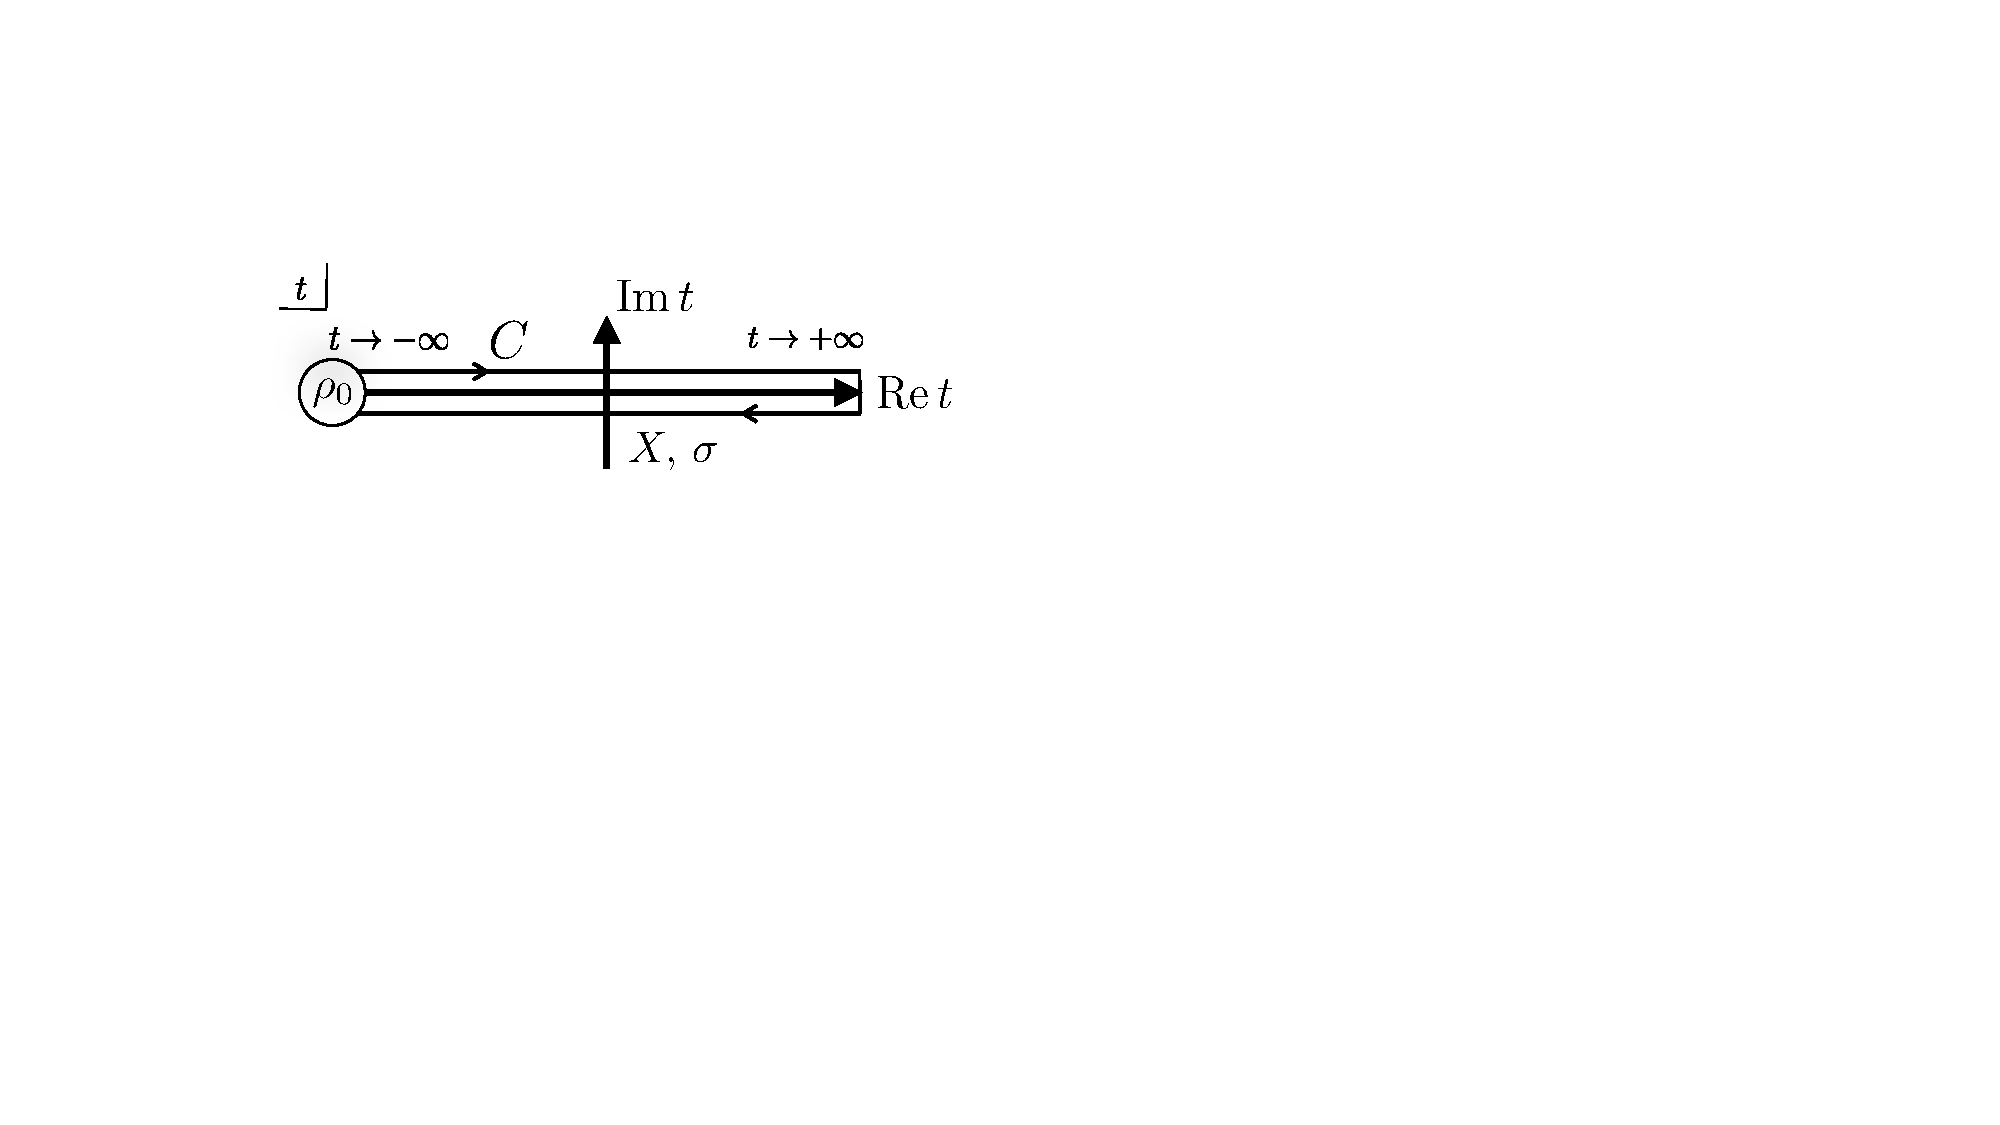
\includegraphics[width=8cm]{original/fig_ctp_x}
\caption{
生成汎関数が定義される閉時間経路。
初期密度演算子 $\hat{\rho}_0$ が熱的密度演算子 $\hat{\rho}_0 \propto e^{-\beta \hat{H}}$ で与えられると仮定すると、負の虚時間方向へ延びる別の経路が存在する（付録\ref{kim}を参照）。}
 
\label{fig:CTP}
\end{center}
\end{figure}


\medskip
微視的作用 $S_{\rm micro}$ が時間並進対称性を持つとき、式\eqref{pi_micro}の指数部は、$\epsilon_a~(a=1,2)$ でラベル付けされる二重化された時間並進\footnote{
正確には、$\epsilon_1\neq\epsilon_2$ の変換は、先に述べた $1$ と $2$ の変数間の $\mathcal{O}(\epsilon)$ の混合によって破られる。ここで、添字 $a=1,2$ の付かない $\epsilon$ は、$i\epsilon$ 処方の無限小パラメータである。}の下で不変である。
\begin{align}
 X_1(t) \to X'_1 (t) = X_1 (t+\epsilon_1)
 \,,
 \quad
 X_2(t)\to X'_2 (t) = X_2 (t+\epsilon_2)
\end{align}
$\sigma_a$ と $J_a$ にも同様の変換則がある。これは、$a=1$ の変数と $a=2$ の変数が分離しているためである。
以下で詳しく述べるように、これら二つの対称性の組合せが、前小節で述べた $\hat{H}_{R}$ と $\hat{H}_A$ に伴う二つの対称性になる。
次に、環境 $\sigma$ を積分消去すると、この対称性構造がどのように変化するかを議論する。
ここで重要なのは、$\sigma_1$ と $\sigma_2$ の間に、オンシェル粒子の生成に関連する非自明な相関が存在するという点である。
その結果、Brown粒子 $X_a$ が環境に結合していると、$\sigma_a$ を積分消去した後の有効作用は、$a=1$ の部分と $a=2$ の部分に分離できない。
\begin{align}
 Z[J_1,J_2]=\int \mathcal{D} X_1 \mathcal{D} X_2 
 \exp \Big[iS_{\rm eff}[X_1,X_2;J_1,J_2] \Big]
 \,.\label{eq:MSR10}
\end{align}

\begin{figure}[t]
 \begin{center}
  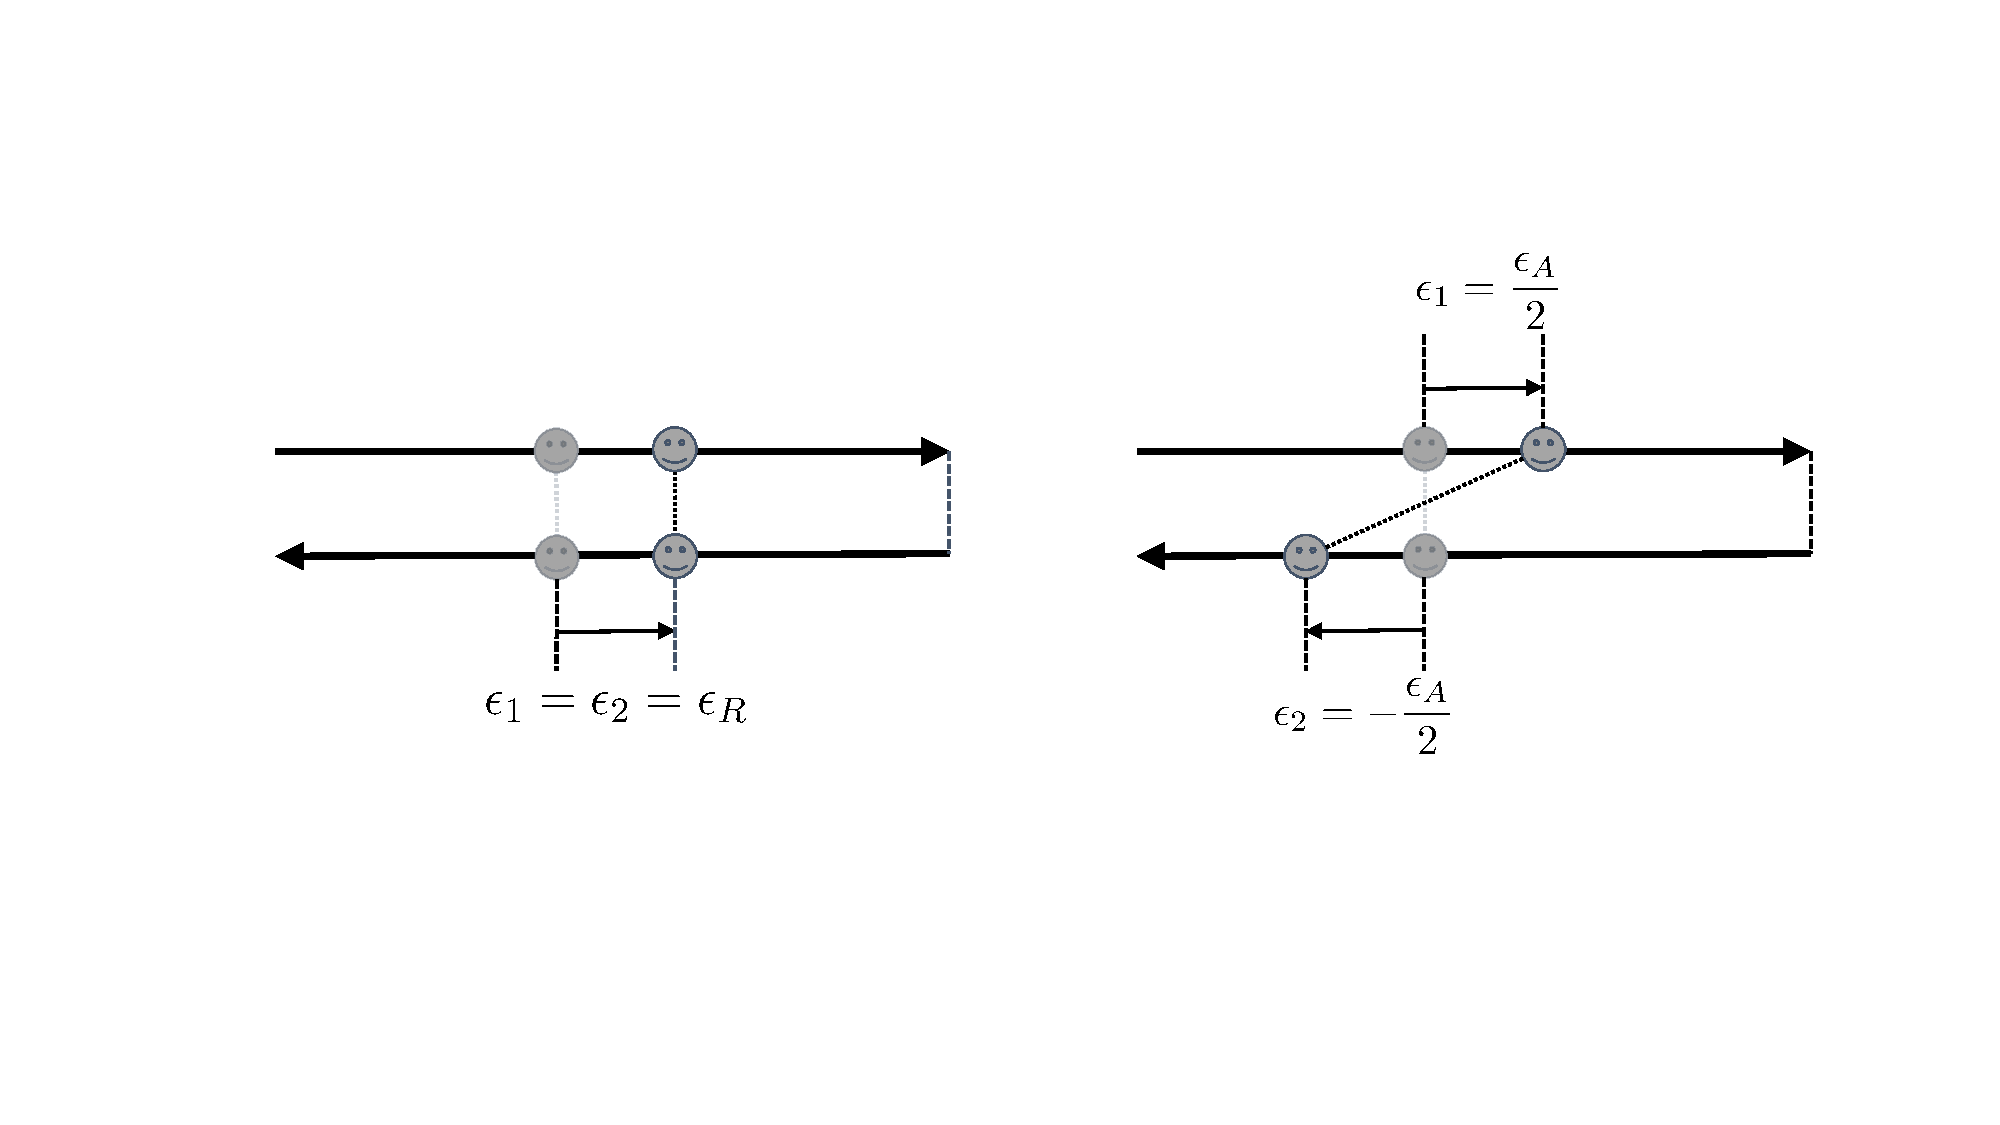
\includegraphics[width=15cm]{original/fig_eRA}
  \caption{
閉時間経路上の $\epsilon_{R}$ 変換と $\epsilon_{A}$ 変換。
$\epsilon_{R}$ は $a=1,2$ の変数を同じ方向に並進させる一方、$\epsilon_{A}$ は逆方向に並進させる。
$t$ に陽に依存しない Lagrangian は、$\epsilon_{R}$ 並進の下でのみ不変である。
右図に示すように、同時刻の $1$--$2$ 結合は、$\epsilon_A$ 変換を行うと、もはや同時刻の結合ではなくなる。}
  \label{fig:TwoTimeTr}
 \end{center}
\end{figure}


よく知られた具体例を調べ、Brown粒子に対する $S_{\mathrm{eff}}[X_1,X_2]$ を具体的に求めよう。
軽い調和振動子 $\sigma (t) =\{x_1 (t), \cdots, x_N(t)\}$ と結合した一次元の Brown点粒子 $X(t)$ を考える。その全作用は、次式で与えられる。
\begin{equation}
 S_{\mathrm{total}}[X,\{x_n\}] 
  = \int dt 
  \Big[ L_{\mathrm{sys}} + L_{\mathrm{env}} + L_{\mathrm{int}} \Big] .
  \label{eq:TotalL}
\end{equation}
ここで、$L_{\mathrm{sys}},\, L_{\mathrm{env}}$ および $L_{\mathrm{int}}$ は、それぞれ Brown粒子、環境の調和振動子、およびそれらの相互作用に対する Lagrangian を表す。
\begin{equation}
 L_{\mathrm{sys}} 
  = \dfrac{M}{2} \dot{X}^2 - V (X), 
  \quad
  L_{\mathrm{env}} 
  =  \displaystyle{\sum_{n=1}^N }
  \left[ \dfrac{m_n}{2} \dot{x}_n^2 - \dfrac{1}{2} m_n \omega_n^2 x_n^2 \right], 
  \quad
  L_{\mathrm{int}} 
  =  \displaystyle{\sum_{n=1}^N} g_nx_n X , 
  \label{eq:EachL}
\end{equation}
$m_n$ と $\omega_n$ は、それぞれ環境の第 $n$ 調和振動子の質量と振動数である。
簡単のため、$X$ と $x_n$ の間には、結合定数 $g_n$ を持つ線形結合を導入した。
環境には、いわゆる\textit{Ohmic 浴}~\cite{kamenev2011field}を用いる。これは連続スペクトルを持つので、$N$ は非常に大きい（詳細は付録\ref{kim}を参照）。
また、初期時刻（$t=-\infty$）では熱平衡にあると仮定する。
付録\ref{kim}では、この Lagrangian から出発して、重い粒子に対する次の有効作用を導出する。
\begin{align}
 iS_{\mathrm{eff}} [X_1,X_2] 
 = i\int dt\, 
 &\left[ - \frac{M}{2} X_{i} D^{-1}_{ij} X_{j} - V(X_1) + V(X_2) \right], 
 \label{eq:MSR3}
\end{align}
ここで、次のように定義した。
\begin{align}
 D^{-1}_{ij}
 = \begin{pmatrix}
    \partial_{t}^{2}-\dfrac{iA}{M} & \gamma\partial_{t} + \dfrac{iA}{M} 
    \vspace{5pt} \\
    - \gamma\partial_{t} + \dfrac{iA}{M} & - \partial_{t}^{2} - \dfrac{iA}{M}
   \end{pmatrix}
   \quad
   {\rm with}
   \quad
   A=2M\gamma/\beta
   .
  \label{D-1}
\end{align}
ここで、$\gamma$（$>0$）は、Ohmic 浴における調和振動子の振動数分布を特徴付けるパラメータである。
熱平衡を仮定したため、FDR $A=2M\gamma/\beta$ が満たされていることに注意しよう。
予想したとおり、環境 $x_n$ を積分消去すると混合項が生じ、$a=1,2$ の変数は互いに結合する。
この混合項により、有効作用は $\epsilon_1 \neq \epsilon_2$ という選択の下では、もはや不変ではない。
したがって、有効作用の対称性は、次のようにパラメータを制限した時間並進対称性となる（図\ref{fig:TwoTimeTr}の左図を参照）。
\begin{align}
\label{eR}
 \epsilon_1 = \epsilon_2 = \epsilon_R 
 \,,
\end{align}
ここで、共通のパラメータを $\epsilon_R$ と表した。
また、後で用いるため、（陽に）破れた対称性も $\epsilon_A$ を用いて次のように表す（図\ref{fig:TwoTimeTr}の右図を参照）。
\begin{align}
\label{eA}
 \epsilon_1 = - \epsilon_2 = \frac{\epsilon_A}{2} \,.
\end{align}
このように、ゆらぎと散逸が存在すると、微視的作用の二つの時間並進対称性は、対角的な対称性 $\epsilon_1=\epsilon_2$ へと破れる。
これは、まさに前小節で見たことである。



\medskip
前小節の議論との関係をより明確に見るには、次の新しい基底を導入すると便利である。
\begin{align}
 X_R = \frac{X_1 + X_2}{2}\,,
 \quad
 X_A= X_1 - X_2  \,.
\end{align}
$\epsilon_R$ をパラメータとする変換\eqref{eR}の下で、これらは次のように変換する。
\begin{align}
 \begin{cases}
  X_R(t) \to X'_R (t) = X_R (t+\epsilon_R)\,, \\
  X_A(t) \to X'_A(t) = X_A (t+\epsilon_R)\,,
 \end{cases}
\end{align}
$X_{R}$ と $X_A$ を MSR 形式の同名の変数と同一視すると、これはまさに、Fokker-Planck Hamiltonian が生成する $H_A$ 変換\eqref{eq:Timetr1}である。
一方、$\epsilon_A$ をパラメータとする、陽に破れた変換\eqref{eA}は、次の形を取る。
\begin{equation}
  \begin{cases}
   X_R(t) 
   \to X'_{R}(t) 
   = X_R(t)+ \dfrac{1}{4} \epsilon_A \dot{X}_A(t) + O (\epsilon_A^2) \,,
   \vspace{5pt} \\
   X_A(t) 
   \to X'_A(t) 
   = X_A(t) +\epsilon_A\dot{X}_R+ O (\epsilon_A^2)\,.
  \end{cases}
\end{equation}
ここで、$X_{R} =O (\hbar^0)$ および $X_A = O(\hbar)$ となるように $\hbar$ 依存性を割り当てると便利である。
すると、半古典極限（$\hbar\to0$）において、上の変換は次の形に帰着する。
\begin{equation}
 \begin{cases}
  X_R(t) \to 
  X'_R(t) = X_R(t) + O(\epsilon_A^2)\,,
  \\
  X_A(t)\to 
  X'_A(t) = X_A(t) + \epsilon_A \dot{X}_{R} + O(\epsilon_A^2)\,,
 \end{cases}
\end{equation}
その最低次の部分は、まさに Brown粒子のもとの Hamiltonian が生成する $H_R$ 変換\eqref{eq:Timetr2}である。
これは、MSR 有効作用が Schwinger-Keldysh 作用の半古典極限として得られることを意味する。
\medskip

まとめると、Schwinger-Keldysh 形式における微視的（UV）作用は、閉時間経路という性質のためにすべての場が二重化されるのと同様に、$\epsilon_R$ と $\epsilon_A$ でラベル付けされる二重化された時間並進対称性を持つ。
しかし、環境を積分消去した後の有効（IR）作用には、$a=1,2$ の変数間の混合が含まれ、これは確率的効果および散逸効果と解釈される。
このような混合は、二重化された対称性を、$\epsilon_R$ でラベル付けされる対角的な対称性へと陽に破る。この対称性は、まさに Fokker-Planck Hamiltonian が生成する $H_A$ 時間並進変換である。
一方、$\epsilon_A$ でラベル付けされる陽に破れた対称性は、半古典極限（$\hbar \to 0$）において、Brown粒子の Hamiltonian が生成する $H_R$ 変換と同一視される。
これで、$H_A$ 対称性の自発的破れに基づく有効場理論の観点から、非定常な確率分布を記述する可能性を議論できるようになった。これが、次節で議論する主題である。





\sectionlink{Schwinger-Keldysh形式に基づくEFTの構築}
\label{section:ConstructingEFT}

ここまで、1次元のBrown粒子における対称性の構造を明らかにし、表~\ref{table:ss}にまとめたように、それがSchwinger-Keldyshの観点から自然に理解できることを示した。本節では、これまでの議論、特に$\epsilon_R$で特徴づけられるSSBの\textit{弱い}判定基準を踏まえて、時間依存する凝縮を伴う非平衡状況を、時間並進対称性の破れた相とみなす。\ref{sec:Prelim}節では、まずin-out形式における時間並進対称性の破れの有効Lagrangianと、Schwinger-Keldysh（in-in）形式に基づくEFTの基本的な構築法を概観する。\ref{subsec:EFT_const}節では、対称性の構造に基づいてNambu-Goldstone場の一般的な有効Lagrangianを構築する。NGボソンの分散関係を導出し、動的KMS対称性からEFTに課される制約も考察する。さらに\ref{sec:ModelAnalysis}節では、ノイズと散逸を伴う単一のスカラー場からなる簡単なUV模型を考え、ツリーレベルの解析を行う。この模型解析により、構築したEFTの低エネルギー係数がUV理論の情報とどのように関連するかを示す。本節全体を通じて、特に断らない限り、対称性が破れる前の系はもともとLorentz不変であると仮定する。

\begin{table}[t]
  \centering
  \begin{tabular}{c|cc}
    \hline
    &$H_{A}$対称性&$H_{R}$対称性\\
    \hline \hline
   開放系（定常） & 破れていない & 陽に破れている \\
   開放系（非定常） & 自発的に破れている & 陽に破れている \\
    \hline
  \end{tabular}
 \caption{開放系における対称性の構造。Schwinger-Keldysh形式では対称性が二重化されるため、$H_A$対称性と$H_R$対称性を別々に議論する必要がある。開放系では$H_R$対称性は陽に破れている一方、$H_A$対称性は定常背景では破れておらず、非定常背景では自発的に破れている。これは、全系のHamiltonianによってダイナミクスが記述される、温度ゼロの閉鎖系とは著しく異なる。}
 \label{table:ss}
\end{table}

\subsectionlink{準備}
\label{sec:Prelim}
\ref{subsec:EFT_in-out}節では、まず、宇宙インフレーションの文脈で発展してきた時間並進対称性の破れに対する有効場理論の基本的な構築法をまとめる~\cite{Cheung:2007st}。続いて、Schwinger-Keldysh形式に基づき、このEFTを非平衡状況にある開放系へ拡張する方法を示す。

\subsubsection{in-out形式における有効Lagrangian}
\label{subsec:EFT_in-out}

まず、時間並進対称性の破れに対するin-out有効Lagrangianを簡単に振り返る。時間並進不変な作用$S_{\mathrm{micro}}$をもつ\textit{任意の}UV理論を考え、あるスカラー凝縮$\langle\phi(t,\mathbf{x})\rangle$が非自明な時間依存性をもつと仮定する：
\begin{align}
\label{condensate}
 \langle\phi(t,\mathbf{x})\rangle
 = \bar{\phi}(t)
\quad
{\rm with}
\quad
\dot{\bar{\phi}}\neq0
\,.
\end{align}

この状況では、系の時間並進対称性は明らかに破れている。したがってNGモード$\pi(x)$を、この時間依存する凝縮に次のように埋め込むことができる：
\begin{align}
\label{embedding}
\phi(t,\mathbf{x})=\bar{\phi} \big(t+\pi(t,\mathbf{x}) \big)
\end{align}

このとき、並進の下での変換則は
\begin{align}
 \label{translations}
 \pi(t,\mathbf{x})
 \to \pi'(t,\mathbf{x})
 = \pi(t+\epsilon^0,\mathbf{x}+\boldsymbol{\epsilon})+\epsilon^0\,.
\end{align}

である。さらにLorentz変換の下では、NGモード$\pi(x)$は
\begin{align}
 \label{Lorentz}
 \pi(t,\mathbf{x})
 \to \pi' (t,\mathbf{x}) 
 = \pi \left(\Lambda^0{}_\mu x^\mu,\Lambda^i{}_\mu x^\mu\right)+\Lambda^0{}_\mu x^\mu-t
\,,
\end{align}

と変換する。ここで$\Lambda^\mu{}_\nu\in SO(1,3)$を導入した。NGモードに通常みられるように、$\pi(x)$は、時間依存する凝縮~\eqref{condensate}によって破られる時間並進およびブーストの下で非線形に変換することに注意されたい\footnote{逆Higgs効果~\cite{Ivanov:1975zq}として知られているように（最近の議論については、例えば文献~\cite{Nicolis:2013sga,Endlich:2013vfa,Brauner:2014aha,Hidaka:2014fra}も参照）、質量のないNGボソンの数は、破れた時空対称性の数と必ずしも一致しない。その結果、ブーストに対応するNGボソンを導入せずに、破れたブースト対称性を非線形に実現できる。}。説明のために単一のスカラー凝縮を例にとったが、上の変換則は一般に適用できる。

\medskip
埋め込み~\eqref{embedding}が示唆するように、一般的な有効作用は、次のものから構築される~\cite{Cheung:2007st}：
\begin{align}
 t + \pi(x)
\quad
\text{およびその微分}
\end{align}

実際、これらの構成要素は、適切な座標変換を併せて行えば、変換~\eqref{translations}--\eqref{Lorentz}の下で不変であることを明示的に示せる。有効Lagrangianを構築する際には、
\begin{align}
P_\mu=\partial_\mu(t+\pi)=\delta^0_\mu+\partial_\mu\pi\,,
\label{notation:P}
\end{align}

を導入し、基本的な構成要素として用いると便利である。特に、そのLorentz不変な2乗は
\begin{align}
 P_\mu P^\mu=-1-2\dot{\pi}+(\partial_\mu\pi)^2\,.
\end{align}

となる。微分展開の最低次\footnote{$\pi$に2階以上の微分が作用する高階微分項を省いた。}では、一般的な有効作用は次式で与えられる~\cite{Cheung:2007st}：
\begin{align}
\label{S_in-out_P}
 S_{\text{in-out}} 
 = -\frac{1}{2}\int d^4x 
 \left[ \alpha_0(t+\pi) + \alpha_1(t+\pi) P_\mu P^\mu 
 + \sum_{n\geq2}\alpha_n(t+\pi)(P_\mu P^\mu+1)^n 
\right]\,,
\end{align}

ここで$\alpha_n$は$t+\pi$の任意関数である。内部対称性が破れる場合とは異なり、NGボソン$\pi$は一般にはシフト対称性をもたない。その結果、上の作用には$\pi$について1次の項が含まれる：
\begin{align}
 S_{\text{in-out}} 
 = -\frac{1}{2}\int d^4x 
 \left[ \alpha_0(t) - \alpha_1(t)
 + \Big(\alpha'_0(t)-\alpha'_1(t)\Big)\pi-2\alpha_1(t)\dot{\pi} + O (\pi^2)
\right]\,.
\end{align}

このようなタドポール項を取り除くため、背景の運動方程式を用いて$\alpha'_0=-\alpha'_1$を要求する。すると作用は次のように書き直せる：
\begin{align}
S_{\text{in-out}}=-\frac{1}{2}\int d^4x\left[\alpha_1(t+\pi)(\partial_\mu\pi)^2+\sum_{n\geq2}\alpha_n(t+\pi)\left(-2\dot{\pi}+(\partial_\mu\pi)^2\right)^n
\right]\,,\label{action:pi:inout}
\end{align}

ここでは方程式$\alpha'_0=-\alpha'_1$の積分定数を、$\alpha_0=-\alpha_1$となるように選んだ。これが、破れた時間並進に対応するNGボソンの一般的なin-out有効作用である。

\medskip
ここで強調しておくと、式~\eqref{action:pi:inout}のEFT係数$\alpha_n$は、内部対称性の破れの場合とは異なり、一般には時間に依存する。したがって、関数の自由度があるため、この段階ではEFTの予言能力は限られる。また、時間並進不変性はもはや存在しないので、エネルギーも明確には定義されない。エネルギーを明確に定義し、EFTに普遍的な予言能力を与えるには、さらに別の対称性の仮定を課すと便利である。典型的な例の一つは、秩序変数の時間依存性を無視することである\footnote{別の興味深い状況として、同期現象や時間結晶のように、秩序変数が時間に関して周期的な場合がある。その場合、長時間領域ではエネルギーが明確に定義される。NG場には、空間方向の周期的変調の場合~\cite{Hidaka:2015xza}と同様に、バンド構造が現れるだろう。この問題は別の機会に再び取り上げる。}。宇宙インフレーションとの類似から\footnote{スローロール・インフレーションの間、インフラトン背景の速度$\dot{\bar{\phi}}$はほぼ一定である。その結果、近似的なde Sitter時間並進対称性が存在する。}、このパラメータ領域をスローロール領域と呼ぶ。

\medskip
スローロール領域では$\alpha_n$の時間依存性を無視でき、NGモードの有効作用は次の形に簡単化される：
\begin{align}
 \label{slow-roll_in-out}
 S_{\text{in-out}} 
 = - \frac{1}{2} \int d^4x
 \left[ \alpha_1 (\partial_\mu\pi)^2 + 
 \sum_{n\geq2} \alpha_n \left(-2\dot{\pi} + (\partial_\mu\pi)^2 \right)^n
 \right]\,,
\end{align}

ここで$\alpha_n$は定数パラメータとなり、$\alpha_1$は対称性の破れのスケールを特徴づける。第1項は正準的な運動項に全体の係数$\alpha_1$を掛けただけのものであることに注意されたい。したがって、高次の項$\alpha_n$を有効にしない限り、NGモードは相対論的な分散関係に従い、自己相互作用をもたない。一般には、NGモードは1とは異なる伝播速度をもつ線形分散に従う：
\begin{equation}
 \omega^2 = c_s^2 k^2 \with 
  c_s^2 \equiv \frac{\alpha_1}{ \alpha_1 - 4 \alpha_2}\,.
\end{equation}

以下では、ゆらぎや散逸などの開放系の効果を考慮したとき、この線形分散関係がどのように修正されるかを見る。

\medskip
本小節を終える前に、スローロール領域におけるNGモードの変換特性について述べる。式~\eqref{slow-roll_in-out}からわかるように、スローロール領域ではNGボソンはシフト対称性をもつ。言い換えると、スローロール領域は、$\pi(x)$に対して、並進の下での非線形な変換則~\eqref{translations}の代わりに、次の\textit{線形な}変換則を与えることで実現される：
\begin{align}
 \label{linear_translations}
 \pi(t,\mathbf{x}) 
 \to \pi'(t,\mathbf{x}) 
 = \pi (t + \epsilon^0,\mathbf{x} + \mathbf{\epsilon}) \,,
\end{align}

線形な変換則~\eqref{linear_translations}は通常の物質スカラー場のものと同じなので、有効Lagrangianに$\pi^{n}$も加えられるように思われるかもしれない。しかし、実際にはそうではない。なぜなら、ブーストについては依然として非線形な変換則~\eqref{Lorentz}を課しているからである\footnote{相対論的超流動のNGモードも、変換則~\eqref{linear_translations}および\eqref{Lorentz}に従う。したがって、相対論的な設定では、その有効作用は式~\eqref{slow-roll_in-out}で与えられる。}。その結果、NGモードには常に微分が伴わなければならず、有効作用の構成要素は$t+\pi(x)$の微分となる。別の言い方をすれば、$\partial_{\mu}\pi$は非線形なブースト変換の下で共変ではない。したがって、微分展開の最低次では有効作用は式~\eqref{slow-roll_in-out}で与えられる。

\subsubsection{Schwinger-Keldysh形式に基づくEFTの構築法}
\label{subsec:EFT_in-in}

\ref{micro:origin}節ですでに導入したように、Schwinger-Keldysh形式で最も重要な量は閉時間経路生成汎関数（CTPGF）$Z[J_1, J_2]$である。CTPGFは理論の実時間ダイナミクスに関するすべての情報を含むが、ここで関心があるのは、時間並進対称性の破れに伴う低エネルギーのダイナミクスだけである。そこで、二重化されたNG型モード$\pi_a(x) ~(a=1,2)$を除くすべてのUV自由度を積分消去し、これらのモードのEFTを次のように構築したい：
\begin{align}
\nonumber
  Z[J_1, J_2] 
  &= \mathrm{Tr} \Big[\hat{\rho}_0 \,
  \hat{U}_{J_2}^\dagger(\infty,-\infty)
  \hat{U}_{J_1} (\infty,-\infty) \Big]\,  \\
\nonumber
  &=\int \mathcal{D} \varphi_1 \mathcal{D} \varphi_2
  \mathcal{D} \sigma_1 \mathcal{D} \sigma_2
  \exp \Big[
  iS_{\mathrm{micro}} [\varphi_1,\sigma_1;J_1] 
 - iS_{\mathrm{micro}} [\varphi_2,\sigma_2;J_2] \Big]  
  \rho_0 (\varphi,\sigma) 
  \, \\
  &= \int \mathcal{D} \pi_1 \mathcal{D} \pi_2
  \exp \Big[
  iS_{\mathrm{eff}} [\pi_1,\pi_2;J_1,J_2] \Big]\, .
 \label{eq:CTPGF}
\end{align}

ここで$\varphi$はUV理論の力学的自由度、$\sigma$は存在しうる環境、$J$は外部ソース、$\rho_0$は初期密度演算子を表す。$\hat{U}_{J_1}$と$\hat{U}^\dag_{J_2}$があるため、場はすべて二重化される。二重化されたNGモードの有効作用$S_{\mathrm{eff}} [\pi_1,\pi_2;J_1,J_2]$は、前小節で示したin-out形式と同様に、時間並進対称性が破れた系の普遍的な低エネルギーダイナミクスを捉えることができる。ただし、Schwinger-Keldysh形式の二重化という性質のために、構造がより複雑になることに注意する必要がある。

\medskip
このような構築法は、散逸を伴う相対論的流体力学のEFTを与えるために、近年明らかにされた~\cite{Crossley:2015evo,Glorioso:2017fpd}。その定式化の基礎を簡単にまとめる。重要なのは、CTPGFが満たす以下の基本的性質を保つように、有効作用$S_{\mathrm{eff}} [\pi_1,\pi_2;J_1,J_2]$を構築することである（これらの条件の導出および詳しい議論は、文献~\cite{Crossley:2015evo,Glorioso:2017fpd}を参照）：
\begin{enumerate}
 \item \textbf{ユニタリティ条件：}
       規格化された初期密度演算子$\mathrm{Tr}\,\hat{\rho}_0 = 1$に対して、CTPGF~\eqref{eq:CTPGF}は
\begin{equation}
	Z[J_1 = J ,J_2 = J] = 1 ,
       \end{equation}

を満たす。これは時間発展演算子のユニタリティ$\hat{U}_{J}^\dagger\hat{U}_{J}=1$から従う。
 \item \textbf{共役条件：}
       初期密度演算子$\hat{\rho}_{0}$の自己共役性（$\hat{\rho}_0^\dag = \hat{\rho}_0$）から、
\begin{equation}
	Z^* [J_1, J_2] = Z[J_2, J_1] .
       \end{equation}

が従う。
 \item \textbf{KMS条件（任意）：}
       初期密度演算子が熱的なもの$\hat{\rho}_0 = e^{-\beta \hat{H}}/Z$であるとき、次の追加的な対称性が現れる：
\begin{equation}
       \label{eq_KMS}
	Z [J_1,J_2 ] =  Z [J_1', J_2'] \with 
	 \begin{cases}
	  J_1'(t) = \epsilon_{\mathcal{T}_J} J_1 (-t + i \beta /2) , \\
	  J_2'(t) = \epsilon_{\mathcal{T}_J} J_2 (-t - i\beta/2) ,
	 \end{cases}
       \end{equation}

ここで$\epsilon_{\mathcal{T}_J}$は、$J$に結合する演算子の、時間反転（必要ならパリティ変換も同時に行う）の下での固有値を表す。
\end{enumerate}
最初の二つの条件は非常に一般的だが、最後の条件には初期密度演算子$\rho_0$に対する強い仮定が必要なので、これを任意の条件として扱うことに注意されたい。

\medskip
次に問題となるのは、これらの性質に基づいてEFTの構造をどのように制限するかである。上の条件が確実に満たされるように、有効作用$S_{\mathrm{eff}} [\pi_1,\pi_2;J_1,J_2]$にいくつかの仮定を置く。簡単のため、以下では外部ソースを省くが、それらを含めることも容易である。ユニタリティ条件と共役条件は、次を課すことによって$S_{\mathrm{eff}} [\pi_1,\pi_2]$に実装できる：
\begin{align}
 S_{\mathrm{eff}} [\pi,\pi] &=0 ,\label{+-unitary:action}
 \\
 S_{\mathrm{eff}} [\pi_1,\pi_2]& = -S[\pi_2,\pi_1]^*,
\label{+-unitarity:2}
\end{align}

ここで$S[\pi_1,\pi_2]^*$は$S[\pi_1,\pi_2]$の複素共役を表す。第2の関係~\eqref{+-unitarity:2}は、一般に有効作用が虚部をもつことを示している。環境（UV）の自由度を積分消去した後のダイナミクスは一般にゆらぎと散逸を含むので、これは開放系の基本的な特徴である。経路積分の重みが$e^{iS_{\mathrm{eff}}}$であることを思い出すと、$\mathrm{Im} S_{\mathrm{eff}} < 0$の場合にはCTPGFが発散する可能性がある。この問題を避けるため、有効作用の虚部の正値性も課す\footnote{正値性条件の導出については文献~\cite{Glorioso:2016gsa}を参照。}：
\begin{align}
 \mathrm{Im} S_{\mathrm{eff}} [\pi_1,\pi_2] \geq 0.\label{unitary:open}
\end{align}

次で定義される$RA$基底を導入することも便利である：
\begin{align}
 \pi_R = \frac{\pi_1 + \pi_2}{2}\,,
 \quad
 \pi_A=\pi_1-\pi_2\,.
\label{def:RAbasis}
\end{align}

すると、有効作用に対するユニタリティ条件および共役条件~(\ref{+-unitary:action})、(\ref{+-unitarity:2})は、
\begin{align}
S[\pi_{R},\pi_{A}=0]&=0,\label{unitary:action}
\\
S[\pi_{R},\pi_{A}]&=-S [\pi_{R},-\pi_{A}]^*,
\label{unitarity:2}
\end{align}

と書き直せる。次小節ではこれらを用いる。KMS条件からEFTに制約を課すこともできる。しかし、KMS条件はEFTに現れることも現れないこともあるため、この問題については、次小節で一般的な有効Lagrangianを構築した後に議論する。

\subsectionlink{開放系における有効Lagrangian}
\label{subsec:EFT_const}

次に、開放系におけるNGモードのEFTを構築する。\ref{micro:origin}節で詳しく述べたように、Schwinger-Keldysh形式では、すべての微視的な対称性が二重化される。非線形な変換則~\eqref{translations}--\eqref{Lorentz}に対応して、二重化されたNGモードの、二重化されたPoincar\'e対称性の変換は、次で与えられる（$a=1,2$）：
\begin{align}
\label{pi_a_translations}
 \pi_a(t,\mathbf{x})
 &\to \pi_a'(t,\mathbf{x})
 = \pi_a\left(t+\epsilon^0_a,\mathbf{x}+\boldsymbol{\epsilon}_a\right)+\epsilon^0_a\,,
\\
\pi_a(t,\mathbf{x})
 &\to \pi_a' (t,\mathbf{x}) 
 = \pi_a \left(\Lambda_a^0\,{}_\mu x^\mu,\Lambda_a^i\,{}_\mu x^\mu\right)+\Lambda_a^0\,{}_\mu x^\mu-t
\,,
\end{align}

ここで$\epsilon_a$および$\Lambda_a^\mu\,{}_\nu\in SO(1,3)$は、それぞれ二重化された並進対称性とLorentz対称性の変換パラメータである。特に、開放系であることにより、二重化された対称性は対角的なもの、すなわち$\epsilon_1=\epsilon_2=\epsilon_R$および$\Lambda_1=\Lambda_2=\Lambda_R$へと陽に破れる。ここから先では、この二つを$\epsilon_R$対称性と$\Lambda_R$対称性と呼ぶ。なお前節では、$\epsilon_R$対称性を$H_A$対称性と呼んでいた。また、破れた対称性を$\displaystyle\epsilon_1=-\epsilon_2=\frac{\epsilon_A}{2}$および$\Lambda_1=(\Lambda_2)^{-1}=(\Lambda_A)^{1/2}$とパラメータ化し、それらを$\epsilon_A$対称性および$\Lambda_A$対称性と呼ぶ。$RA$基底~\eqref{def:RAbasis}では、NGモードの$\epsilon_R$変換は
\begin{align}
\label{R_translations_R}
 \pi_R(t,\mathbf{x})
 &\to \pi_R'(t,\mathbf{x})
 = \pi_R\left(t+\epsilon^0_R,\mathbf{x}+\boldsymbol{\epsilon}_R\right)+\epsilon^0_R\,,
\\
\label{R_translations_A}
  \pi_A(t,\mathbf{x})
 &\to \pi_A'(t,\mathbf{x})
 = \pi_A\left(t+\epsilon^0_R,\mathbf{x}+\boldsymbol{\epsilon}_R\right),
\end{align}

であり、$\Lambda_R$変換は次で与えられる：
\begin{align}
\label{R_Lorentz_R}
\pi_R(t,\mathbf{x})
 &\to \pi_R' (t,\mathbf{x}) 
 = \pi_R \left(\Lambda_R^0\,{}_\mu x^\mu,\Lambda_R^i\,{}_\mu x^\mu\right)+\Lambda_R^0\,{}_\mu x^\mu-t\,,
 \\
\label{R_Lorentz_A}
 \pi_A(t,\mathbf{x})
 &\to \pi_A' (t,\mathbf{x}) 
 = \pi_A \left(\Lambda_R^0\,{}_\mu x^\mu,\Lambda_R^i\,{}_\mu x^\mu\right)\,.
\end{align}

ここで重要なのは、$\pi_A$場が、通常の物質場と同じように、$\epsilon_R$対称性および$\Lambda_R$対称性の下で\textit{線形に}変換することである。同様に、$\pi_{R/A}$場は$\epsilon_A$対称性および$\Lambda_A$対称性の下で、それぞれ線形／非線形に変換することがわかる（$RA$基底での変換則は、後で必要になったときに明示する）。以下では、この対称性の構造と、\ref{subsec:EFT_in-in}節でまとめたSchwinger-Keldysh条件に基づき、二重化されたNGモードの有効Lagrangianを構築・解析する。

\subsubsection{一般的なLagrangian}

先ほど述べたように、$\epsilon_R$対称性および$\Lambda_R$対称性の観点からは、$\pi_A$場を物質場とみなせる。したがって、$\epsilon_R$対称性と$\Lambda_R$対称性のみを保つ、開放系の有効作用の一般的な構成要素は、次で与えられる：
\begin{align}
\pi_{A},~t+\pi_{R} \quad\text{およびそれらの微分},
\label{ingredients}
\end{align}

これらはin-outの場合と同様に、適切な座標変換を併せて行えば、式~\eqref{R_translations_R}--\eqref{R_Lorentz_A}の下で不変である。これらの構成要素に基づき、正値性条件~\eqref{unitary:open}、ユニタリティ条件~(\ref{unitary:action})および共役条件~(\ref{unitarity:2})と整合的な、一般的なLagrangianを構築する。

\paragraph{$\hbar$展開}
まず、$RA$場の$\hbar$依存性が次のように与えられることを思い出そう：
\begin{align}
\pi_R=\mathcal{O}(\hbar^0)\,,
\quad
\pi_A=\mathcal{O}(\hbar)\,.
\end{align}

すると、有効Lagrangianは$\hbar$について次のように展開できる：
\begin{align}
\mathcal{L}_{\rm eff}=\sum_{n=1}^\infty \mathcal{L}_n
\quad
{\rm s.t.}
\quad
\mathcal{L}_n=\mathcal{O}(\pi_A^n)=\mathcal{O}(\hbar^n)\,,
\end{align}

ここで、$\hbar$展開は$\pi_A$の個数についての展開に対応し、ユニタリティ条件~\eqref{unitary:action}のために、Lagrangianは$\pi_A$の1次の項から始まることに注意されたい。また、共役条件~(\ref{unitarity:2})は、$n$が奇数（偶数）の$\mathcal{L}_n$に現れる演算子の係数が実数（純虚数）であることを要求する。後で見るように、最低次のLagrangian $\mathcal{L}_1$は散逸項を含み、2次のLagrangian $\mathcal{L}_2$はノイズ項を含む。$\mathcal{O}(\hbar^2)$で展開を打ち切ることを半古典極限と呼ぶ。これはMSR作用のレベルで議論することと等価である。$\hbar$のより高次への構築の拡張は容易だが、以下では技術的に簡単にするため、この半古典極限を用い、$\mathcal{L}_1$と$\mathcal{L}_2$だけを構築する。

\paragraph{$\mathcal{L}_1$の具体例}

まず最低次の$\mathcal{L}_1$から始める。一般的なLagrangianを考える前に、以下の簡単な例を考えると理解しやすい：
\begin{align}
\mathcal{L}_1^{\rm simple}&=
\gamma_0(t+\pi_R)\pi_A
+\gamma_1(t+\pi_R)(P_\mu P^\mu+1)\pi_A
 -\alpha_1(t+\pi_R)P^\mu\partial_\mu\pi_A\,,
 \label{Eq:SimpleL}
\end{align}

ここで$P_\mu=\partial_\mu(t+\pi_R)=\delta_\mu^0+\partial_\mu\pi_R$を導入した。in-outの場合と同様に、EFTパラメータ$\gamma_0$、$\gamma_1$、$\alpha_1$は$t+\pi_R$の関数であり、共役条件~(\ref{unitarity:2})のために実数値でなければならない。また、このLagrangianは$\pi$について1次の項を含む：
\begin{align}
\mathcal{L}_1^{\rm simple}&=\gamma_0(t)\pi_A+\alpha_1(t)\dot{\pi}_A+\mathcal{O}(\pi^2)\,,
\end{align}

そこで、$\pi_A$の背景の運動方程式を課して$\gamma_0=\alpha_1'$を要求する。すると、Lagrangian~\eqref{Eq:SimpleL}は次の形になる：
\begin{align}
\mathcal{L}_1^{\rm simple}
&=
\gamma_1(t+\pi_R)\left(-2\dot{\pi}_R+(\partial_\mu\pi_R)^2\right)\pi_A
-\alpha_1(t+\pi_R)\partial_\mu\pi_R\partial^\mu\pi_A
-\alpha_1'(t+\pi_R)\dot{\pi}_R\pi_A\,,
\end{align}

ここでは全微分を省いた。これらの演算子を直感的に理解するには、EFTパラメータ$\alpha_1$と$\gamma_1$が定数となるスローロール領域を考えると有用である：
\begin{align}
\mathcal{L}_1^{\rm simple}
&=
\gamma_1\left(-2\dot{\pi}_R+(\partial_\mu\pi_R)^2\right)\pi_A
-\alpha_1\partial_\mu\pi_R\partial^\mu\pi_A\,.
\end{align}

例えば式~\eqref{eq:MSR2}との比較からわかるように、$\alpha_1$項はNGボソン$\pi$の通常の運動項である。一方、$\gamma_1$項は散逸項$\dot{\pi}_R\pi_A$を含む。興味深いことに、開放系で時間並進対称性が破れた相では、ブースト対称性を損なうことなく散逸項が現れうる。ブースト対称性は、3次の相互作用項$(\partial_\mu\pi_R)^2\pi_A$を伴うことによって非線形に実現される。

\paragraph{一般的な$\mathcal{L}_1$の構築}

次に、一般的な$\mathcal{L}_1$を考える。in-outの場合~\eqref{S_in-out_P}と同様に、$\pi_{R/A}$に作用する微分が高々1階である演算子に限定しよう。この仮定の下で、一般的なLagrangianは次で与えられる：
\begin{align}
\mathcal{L}_1&=
\mathcal{L}_1^{\rm simple}+\sum_{n=2}^\infty\gamma_n(P^\mu P_\mu+1)^n\pi_A
-\sum_{n=2}^\infty\alpha_n(P^\mu P_\mu+1)^{n-1}P^\mu\partial_\mu\pi_A\,,
\end{align}

ここで$\gamma_n$と$\alpha_n$は$t+\pi_R$の実関数である。$\pi$について1次の項は$\mathcal{L}_1^{\rm simple}$にのみ現れるため、背景の運動方程式は先ほどと同じであることに注意されたい。より具体的には、
\begin{align}
\nonumber
\mathcal{L}_1&=
-\alpha_1(t+\pi_R)\partial_\mu\pi_R\partial^\mu\pi_A
-\alpha_1'(t+\pi_R)\dot{\pi}_R\pi_A
\\
\nonumber
&\quad
-\sum_{n=2}^\infty\alpha_n(t+\pi_R)\left[-2\dot{\pi}_R+(\partial_\mu\pi_R)^2\right]^{n-1}(-\dot{\pi}_A+\partial_\mu\pi_R\partial^\mu\pi_A)
\\
&\quad
+\sum_{n=1}^\infty\gamma_n(t+\pi_R)\left[-2\dot{\pi}_R+(\partial_\mu\pi_R)^2\right]^n\pi_A\,.
\label{EFTLag:pi_A1}
\end{align}

となる。特に、NGモードの分散関係に関わる$\pi$の2次の項を与えるのは、$\alpha_1$、$\alpha_2$、$\gamma_1$の三つの演算子だけである。

\paragraph{$\mathcal{L}_2$の構築}

次に、2次の項$\mathcal{L}_2$に進む。再び、$\pi_{R/A}$に作用する微分が高々1階である演算子に注目しよう。この仮定の下では、分散関係に関わる演算子は四つある：
\begin{align}
\label{L2_simple_P}
\mathcal{L}_2\ni i\Big[
\beta_1\pi_A^2+\beta_2(\partial_\mu\pi_A)^2
+\beta_3(P^\mu\partial_\mu\pi_A)\,\pi_A
+\beta_4(P^\mu\partial_\mu\pi_A)^2
\Big]\,,
\end{align}

ここで$\beta_i$は$t+\pi_R$の実関数である。より具体的には、次のように書ける：
\begin{align}
\nonumber
\mathcal{L}_2&\ni i\Big[
\beta_1(t+\pi_R)\pi_A^2+\beta_2(t+\pi_R)(\partial_\mu\pi_A)^2
+\beta_3(t+\pi_R)(-\dot{\pi}_A+\partial_\mu\pi_R\partial^\mu\pi_A)\pi_A
\\
\nonumber
&\qquad
+\beta_4(t+\pi_R)\big(\dot{\pi}_A^2-2\dot{\pi}_A\partial_\mu\pi_R\partial^\mu\pi_A
+(\partial_\mu\pi_R\partial^\mu\pi_A)^2\big)
\Big]
\\
\label{L2_simple}
&= i\Big[
\big(\beta_1(t) + \tfrac{1}{2}\beta_3'(t)\big)\pi_A^2+\beta_2(t)(\partial_\mu\pi_A)^2
+\beta_4(t)\dot{\pi}_A^2
+\mathcal{O}(\pi^3)\Big]
\,,
\end{align}

ここでは、等号のところで全微分を省いた。また、$\beta_1$と$\beta_3$の演算子は、独立な高次相互作用項を与えるものの、$\pi$の2次のレベルでは縮退していることに注意されたい。

\medskip
式~\eqref{L2_simple}の最終行にある三つの項のうち、第1項は時間依存する係数をもつ通常のノイズ項である。一方、残りの二つは高階微分補正であり、ノイズをスケール依存にする。特に、$\beta_4$項はLorentz対称性を破るため、自発的に破れたブースト対称性を非線形に実現するには、3次および4次の相互作用項を伴わなければならない。同様に、$\mathcal{L}_2$の一般的な演算子は、上に示した四つの演算子に$(P_\mu P^\mu+1)=-2\dot{\pi}_R+(\partial_\mu\pi_R)^2$の任意のべきを掛けることで得られる。これらの新しい演算子は3次以上の相互作用項を生成するため、分散関係には関わらず、弱結合領域では劣位の寄与でもある。

\medskip
すでに述べたように、共役条件~(\ref{unitarity:2})は、偶数$n$の$\mathcal{L}_n$が有効作用の虚部に寄与することを要求する。その符号は正値性条件~\eqref{unitary:open}によって固定される。弱結合領域では、2次の項が3次以上の相互作用よりも支配的なので、虚部への主要な寄与は式~\eqref{L2_simple}の三つの2次の項である。ここで、$\mathcal{L}_n$（$n\geq3$）は、定義により二つより多くの$\pi_A$を含むため、2次の項をまったく与えないことに注意されたい。また、微分展開が有効である限り、第1項が他の項よりも支配的である。これらの仮定の下で、正値性条件~\eqref{unitary:open}は$\beta_1-\tfrac{1}{2}\beta_3'>0$と表せる。

\subsubsection{低エネルギースペクトル}

次に、低エネルギー領域の分散関係を議論する。分散関係を求めるため、EFTパラメータを定数として扱うことができ、エネルギーが明確に定義されるスローロール領域に注目しよう。この領域では、有効Lagrangianの2次の部分は次の形をとる：
\begin{align}
\nonumber
\mathcal{L}_{\rm eff}&\ni
(\alpha_1-2\alpha_2)\dot{\pi}_R\dot{\pi}_A-\alpha_1\partial_i\pi_R\partial_i\pi_A
-2\gamma_1\dot{\pi}_R\pi_A
\\
\label{quadratic_EFT}
&\quad
+i\Big[
\beta_1\pi_A^2-(\beta_2-\beta_4)\dot{\pi}_A^2+\beta_2(\partial_i\pi_A)^2
\Big]\,,
\end{align}

ここで、すべてのEFTパラメータは実定数であり、正値性条件~\eqref{unitary:open}によって$\beta_1>0$が要求される。低エネルギー極限では、以下の演算子が他の演算子よりも支配的となる：
\begin{align}
\nonumber
\mathcal{L}_{\rm eff}&\ni
-\alpha_1\partial_i\pi_R\partial_i\pi_A
-2\gamma_1\dot{\pi}_R\pi_A
+i\beta_1\pi_A^2\,,
\end{align}

ここでは、
\begin{align}
\label{low-energy_assumptions}
\omega\ll\gamma_1/\alpha_i\,,
\quad
\omega^2,k^2\ll|\beta_1/\beta_{2,4}|\,,
\end{align}

を用いて高階微分項を省いた。この二つの条件の物理的解釈は後で示すが、いずれにせよ、十分に低いエネルギースケールを考える限り、これらは満たされる。この低エネルギー極限では、オンシェル条件は次のように表せる：
\begin{align}
{\rm det}\left(
\begin{array}{cc}0 &-\frac{1}{2} \alpha_1k^2- i\gamma_1\omega \\ -\frac{1}{2}\alpha_1k^2+i\gamma_1\omega & i\beta_1\end{array}
\right)=0
\quad
\Leftrightarrow
\quad
\omega^2=-\frac{\alpha_1^2}{4\gamma_1^2}k^4\,.
\end{align}

ここで、ノイズ項$\beta_1$は分散関係に影響しないことに注意されたい。興味深いことに、二重化されたNGモードは正準共役対を形成し、2次の分散をもつ単一の\textit{拡散}モードを記述する。これは閉鎖系のNGモードとは著しく異なる。開放系におけるNGモードのこのような分散関係は、内部対称性の破れの場合について以前に見いだされている~\cite{Minami:2018oxl}。本研究の設定で拡散モードと2次分散が現れる起源は、そこで議論された内部対称性の破れの場合と本質的に同じである。

\subsubsection{エネルギースケール}

ここで、低エネルギー極限をとるために用いた二つの条件~\eqref{low-energy_assumptions}に戻ろう。まず、第2の条件は容易に理解できる。これは、ノイズ効果を生成する演算子の間で微分展開が有効であることを要求しているだけである。一方、第1の条件にはもう少し考察が必要である。説明したように、$\gamma_1$演算子は散逸項であるのに対し、$\alpha_1$演算子は通常の運動項である。したがって、第1の条件は、散逸項が時間方向の運動項よりも支配的であることを意味する。言い換えると、この条件は散逸効果のエネルギースケール$E_{\rm diss}$を、次のように特徴づける：
\begin{align}
E_{\rm diss}\sim\gamma_1/\alpha_1\,.
\end{align}

したがって、上で議論した低エネルギー極限は$\omega\ll E_{\rm diss}$と表せる。ここで、時間並進対称性の破れのスケール$E_{\rm SSB}$が、
\begin{align}
E_{\rm SSB}^4\sim \alpha_1\,.
\end{align}

によって特徴づけられることを思い出そう。散逸効果と対称性の破れは異なる起源をもつので、二つのスケール$E_{\rm diss}$と$E_{\rm SSB}$は一般に独立である。特に、階層性$E_{\rm diss}\ll E_{\rm SSB}$が存在すれば、$E_{\rm diss}\ll \omega\ll E_{\rm SSB}$を満たすスケール$\omega$があり、この領域ではNGモードのダイナミクスに対する散逸効果は劣位の寄与となる。したがって、低エネルギー極限を超えて考える場合には、どの演算子が散逸効果に関連しているのか、さらに一般に、どの演算子が開放系に特有なのかを明らかにすることが重要になる\footnote{逆の階層性$E_{\rm SSB}\ll \omega\ll E_{\rm diss}$の場合、EFTによる記述はもはや適用できず、元のUV理論において単にゆらぎと散逸が存在する。}。

\medskip
この動機に基づき、EFTの演算子を分類しよう。まず、$\mathcal{L}_1$と$\mathcal{L}_2$は$\hbar$展開の異なる次数にある。$\mathcal{L}_2$が純虚数であることからわかるように、これは統計的ノイズを記述するので、開放系に特有のものである。一方、$\mathcal{L}_1$には、開放系に特有の演算子と、閉鎖系にも存在しうる演算子の両方が含まれる。\ref{micro:origin}節で議論したように、後者の演算子は$\epsilon_A$対称性と$\Lambda_A$対称性をもつ。特に、二重化されたNGモードの$\epsilon_A$時間並進対称変換は、式~\eqref{pi_a_translations}で$\epsilon^0_1=-\epsilon^0_2=\epsilon_A/2$とおくことで、次のように与えられる：
\begin{align}
\label{epsilon_A_R}
 \pi_R(t,\mathbf{x})&\to 
 \pi'_R(t,\mathbf{x}) 
 = \pi_R(t,\mathbf{x}) 
 +\mathcal{O}(\hbar^2)\,,
 \\
\label{epsilon_A_A}
 \pi_A(t,\mathbf{x})&\to 
 \pi'_A(t,\mathbf{x})
 =\pi_A(t,\mathbf{x})+\dot{\pi}_R(t,\mathbf{x})\epsilon_A+\epsilon_A+ O(\hbar^3)\,,
\end{align}

ここでは、変換パラメータ$\epsilon_A$の$\hbar$依存性を$\epsilon_A=\mathcal{O}(\hbar)$とした。この次数で打ち切ることは、Schwinger-Keldysh作用の半古典極限、すなわちMSR有効作用と整合的であることに注意されたい。次に、$\mathcal{L}_1$の$\epsilon_A$変換を考える。簡単のため、スローロール領域に注目しよう：
\begin{align}
\mathcal{L}_1&=
\sum_{n=1}^\infty\gamma_n(P^\mu P_\mu+1)^n\pi_A
-\sum_{n=1}^\infty\alpha_n(P^\mu P_\mu+1)^{n-1}P^\mu\partial_\mu\pi_A
\,,
\end{align}

ここで$\alpha_n$と$\gamma_n$は定数である。次の変換特性に注意すると、
\begin{align}
\delta_{\epsilon_A} (P^\mu\partial_\mu\pi_A)=\epsilon_A\,P^\mu\partial_\mu(\dot{\pi}_R+1)=\frac{1}{2}\epsilon_A\,\partial_t(P^\mu P_\mu+1)\,,
\end{align}

$\mathcal{L}_1$の$\epsilon_A$変換は次のように計算できる：
\begin{align}
\delta_{\epsilon_A} \mathcal{L}_1&=
\epsilon_A\left[
\sum_{n=1}^\infty\gamma_n(P^\mu P_\mu+1)^n(\dot{\pi}_R+1)
-\sum_{n=1}^\infty\alpha_n\frac{1}{2n}\partial_t(P^\mu P_\mu+1)^{n}
\right]
\,.
\end{align}

第2項は全微分なので、$\alpha_n$演算子は$\epsilon_A$時間並進の下で不変であることがわかる\footnote{\label{footnote:non-slow_roll}スローロールの仮定を緩めた場合、$\alpha_n'= - 2n\gamma_n$と選ぶことで、$\epsilon_A$不変な演算子が与えられる。}。これらが$\Lambda_A$対称性ももつことを示せる。したがって、$\alpha_n$演算子は閉鎖系にも存在しうる一方、$\gamma_n$演算子は開放系に特有である。対応するEFT係数は、次のように見積もられる：
\begin{align}
\alpha_n\sim E_{\rm SSB}^4\,,
\quad
\gamma_n\sim E_{\rm diss}\,E_{\rm SSB}^4\,.
\end{align}

\medskip
最後に、低エネルギー極限を超えて有効な分散関係を導出する。階層性$E_{\rm diss}\ll E_{\rm SSB}$があり、低エネルギー極限での結果がもはや適用できない中間スケール$E_{\rm diss}\lesssim \omega\ll E_{\rm SSB}$が存在すると仮定しよう。この中間スケールでは、2次のLagrangian~\eqref{quadratic_EFT}において、次の演算子が主要な演算子となりうる：
\begin{align}
\nonumber
\mathcal{L}_{\rm eff}&\ni
(\alpha_1-2\alpha_2)\dot{\pi}_R\dot{\pi}_A-\alpha_1\partial_i\pi_R\partial_i\pi_A
-2\gamma_1\dot{\pi}_R\pi_A+i\beta_1\pi_A^2
\\
&=
(\alpha_1-2\alpha_2)\left(
\dot{\pi}_R\dot{\pi}_A-c_s^2\partial_i\pi_R\partial_i\pi_A
-\gamma\dot{\pi}_R\pi_A+i\frac{A}{2}\pi_A^2
\right)
\,,
\label{eq:lag_eff_intscale}
\end{align}

ここでは、ノイズ項に対する高階微分補正を省いた。また、
\begin{align}
c_s^2=\frac{\alpha_1}{\alpha_1-2\alpha_2}\,,
\quad
\gamma=\frac{2\gamma_1}{\alpha_1-2\alpha_2}\,,
\quad
A=\frac{2\beta_1}{\alpha_1-2\alpha_2}\,,
\end{align}

を導入した。ここで$\gamma\sim E_{\rm diss}$と$A$は、それぞれ減衰係数とノイズの振幅である。また、$c_s$はNGモードの伝播速度を表す。分散関係は、
\begin{align}
{\rm det}\left(
\begin{array}{cc}0 &\omega^2-c_s^2k^2- i\gamma\omega \\ \omega^2-c_s^2k^2+ i\gamma\omega & iA\end{array}
\right)=0
\quad
\Leftrightarrow
\quad
\omega^2=c_{s}^{2}k^2-\frac{\gamma^2}{2}\pm\sqrt{\frac{\gamma^4}{4}-\gamma^2c_{s}^{2}k^2}\,.
\end{align}

となる。低エネルギー極限$c_{s}k\ll\gamma\sim E_{\rm diss}$では、ギャップのない拡散モードとギャップをもつ拡散モードが一つずつ得られる：
\begin{align}
\omega^2\simeq- \frac{c_{s}^{4}k^4}{\gamma^2}\,,
\quad
\omega^2\simeq-  \gamma^2+2c_{s}^{2}k^2\,,
\end{align}

ここで、先ほどの議論では低エネルギー極限をとることにより時間方向の運動項$\dot{\pi}_R\dot{\pi}_A$を無視したため、ギャップをもつモードを捉えられなかったことに注意されたい。一方、$c_{s}k\gg \gamma\sim E_{\rm diss}$を満たす短い長さスケールでは、小さな散逸を伴う二つの伝播モードが得られる：
\begin{align}
\omega^2\simeq c_{s}^{2}k^2\pm i \gamma c_{s}k\,.
\end{align}

\subsubsection{動的KMS対称性からEFTへの制約}
\label{subsec:KMS}

\ref{subsec:KMS_B}節で議論したように、系が初期に熱平衡状態にある場合、KMS対称性と呼ばれる追加的な離散対称性が現れる。本小節の残りでは、この対称性が有効作用の低エネルギー係数に及ぼす帰結を議論する。

\paragraph{KMS変換}

\medskip
\ref{subsec:KMS_B}節では、動的KMS変換を、純虚数の変換パラメータ$\epsilon_A=-i\beta$（$\beta$は逆温度）をもつ$\epsilon_A$時間並進~\eqref{epsilon_A_R}--\eqref{epsilon_A_A}と、時間反転変換の組合せとして導入した。NG場のKMS変換を特定するには、時間依存する背景をもつ凝縮場$\phi$を導入すると便利である：
\begin{align}
\langle\phi_a(t,{\bf x})\rangle=\bar{\phi}(t)\,,
\end{align}

ここで$a=1,2$はKeldysh経路上の二重化された場を区別するラベルである。すると、二重化されたNG場$\pi_a$（$a=1,2$）を、次のように埋め込める：
\begin{align}
\phi_a(t,{\bf x})=\bar\phi(t+\pi_a(t,\mathbf x))\,.
\end{align}

凝縮場$\phi$の時間反転パリティが偶であり、
\begin{align}
\phi_a(t,{\bf x})\to\phi_a'(t,{\bf x})=\phi_a(-t,{\bf x})
\quad
(a=1,2)\,,
\label{ota}
\end{align}

ならば、NG場の時間反転変換は次で与えられる：
\begin{align}
\pi_a(t,\mathbf x)\to \pi_a'(t,\mathbf x) = -2t+\pi_a(-t,\mathbf x)\quad
(a=1,2)\,.
\end{align}

$RA$基底では、これを次のように書き直せる：
\begin{align}
    \pi'_R(t,\mathbf x)=-2t+\pi_R(-t,\mathbf x),~~
        \pi'_A(t,\mathbf x)=\pi_A(-t,\mathbf x).
        \label{time:rev}
\end{align}

時間反転対称性はNG場によって非線形に実現されることに注意されたい。その本質的な理由は、時間依存する背景が一般に時間反転対称性を破ることである。

\medskip
したがって、上の時間反転変換と$\epsilon_A$時間並進を用いて、動的KMS変換を導入できる。再び半古典極限をとり、MSR作用のレベルで議論する。パラメータ$\epsilon_A=-i\beta$を用いた式~\eqref{epsilon_A_R}--\eqref{epsilon_A_A}と、式~\eqref{time:rev}から、次の形のKMS変換を得る：
\begin{align}
\label{KMS}
 \pi_R'(t,\mathbf x) =-2t+\pi_R(-t,\mathbf x)
 \,,
 \quad
 \pi_A'(t,\mathbf x) = 
 \pi_A(-t,\mathbf x) 
 + i\beta \big[\partial_{-t} \pi_R(-t,\mathbf x)+1\big]\,,
\end{align}

ここで、$\pi_R$と$\pi_A$の両方が非線形に変換されることに注意されたい\footnote{散逸流体の文脈~\cite{Glorioso:2017fpd}では、非線形な変換~\eqref{KMS}の代わりに、線形なKMS変換則
\begin{align}
\label{dfKMS}
\pi_R'(t,\mathbf x) =-\pi_R(-t,\mathbf x)
 \,,
 \quad
 \pi_A'(t,\mathbf x) = 
 -\pi_A(-t,\mathbf x) 
 - i\beta \partial_{-t} \pi_R(-t,\mathbf x)\,,
\end{align}

がしばしば用いられる。この文脈では、凝縮場$\phi$のパリティは奇であり、定数$v$を用いて$\langle\phi_a(x)\rangle=vt$と書かれるスローロール型の背景をもつ。埋め込み$\phi_a(t,\mathbf x)=v(t+\pi_a(t,\mathbf x))$と、時間反転変換$\phi_a(t,{\bf x})\to\phi_a'(t,{\bf x})=-\phi_a(-t,{\bf x})$から、NG場の動的KMS変換則は次のように従う：
\begin{align}
\label{dfKMS_pre}
 \pi_R'(t,\mathbf x) =-\pi_R(-t,\mathbf x)
 \,,
 \quad
 \pi_A'(t,\mathbf x) = 
 -\pi_A(-t,\mathbf x) 
 - i\beta \big[\partial_{-t} \pi_R(-t,\mathbf x)+1\big]\,,
\end{align}

この段階では、$\pi_R$は線形に変換するが、$\pi_A$は非線形に変換することに注意されたい。さらに、散逸流体では全系のエネルギー保存を実現するために、$\pi_A$のシフト対称性を課す。その結果、$\pi_A$の適切な定数シフトを伴わせることで、非線形な変換~\eqref{dfKMS_pre}を線形な変換~\eqref{dfKMS}へと帰着できる。このように、線形に実現されるKMS対称性を得るには、追加の対称性の存在が決定的に重要である。本論文では、時間並進対称性の破れについてより一般的な設定を考えているため、散逸流体の場合とは異なり、非線形に実現される変換~\eqref{KMS}を採用した。}。

\paragraph{2次のLagrangianへの制約}

次に、動的KMS変換の下での不変性から生じる、任意に課すことのできる制約を議論する。説明のため、EFT係数$\alpha_n, \beta_n, \gamma_n$の時間依存性を無視できるスローロール領域に注目し、KMS不変性がEFTパラメータをどのように制限するかを示す。

\medskip
まず、2次のLagrangian~\eqref{eq:lag_eff_intscale}のKMS変換から始める。最初に、座標変換$t\to-t$を併せて行えば、$\alpha_n$演算子がKMS変換の下で不変であることは容易に示せる。KMS変換と座標変換$t\to-t$の下で、散逸項は次のように変換される：
\begin{align}
 -\gamma\dot{\pi}_R\pi_A 
 &\to \gamma\dot{\pi}_R\pi_A 
 +2\gamma\pi_A+2i\gamma\beta(\dot{\pi}_R+1)
 + i\gamma\beta\dot{\pi}_R(\dot{\pi}_R+1)\,,
\end{align}

一方、ゆらぎの項は次のように変換される：
\begin{align}
 i\frac{A}{2}\pi_A^2 
 \to i\frac{A}{2}\pi_A^2 
-A\beta(\dot{\pi}_R+1)\pi_A
 - i\frac{A\beta^2}{2}(\dot{\pi}_R+1)^2\,.
\end{align}

したがって、減衰係数$\gamma$とノイズの振幅$A$が次の関係を満たすならば、2次のLagrangian~\eqref{eq:lag_eff_intscale}は、全微分を除いてKMS変換~\eqref{KMS}の下で不変となる：
\begin{align}
A=\frac{2\gamma}{\beta}\,,
\end{align}

これは、ほかならぬ揺動散逸関係（FDR）である。正値性条件~\eqref{unitary:open}によって$A>0$が要求されるため、FDRが満たされるならば、減衰係数は正、すなわち$\gamma>0$であることがわかる。

\paragraph{2次のレベルを超えて}

次に相互作用項を取り入れる。ここで非自明なのは、（非線形に実現される）ブースト対称性を保つ限り、散逸項$\dot{\pi}_R\pi_A$には3次の相互作用$\pi_A(\partial_\mu\pi_R)^2$が伴わなければならないことである。FDRが満たされていても、この3次の項$\pi_A(\partial_\mu\pi_R)^2$がKMS変換の下で不変ではないことは容易にわかる。著者らの知る限り、ブースト対称性と動的KMS対称性の両方を保つEFTパラメータの組は存在しない。有限温度の効果はブースト対称性を破るので、このことはそれほど意外ではない。実際、（非線形に実現される時間並進を保ちつつ）ブースト対称性を要求しないことにすれば、有効Lagrangianの構築に$\delta^0_\mu$を用いることができる。例えば、3次の相互作用を伴わずに、散逸項
\begin{align}
\label{Lorentz_breaking_dissipation}
\widetilde{\gamma}_1\left[\delta^0_\mu\partial^\mu(t+\pi_R)\pi_A+\pi_A\right]=-\widetilde{\gamma}_1\dot{\pi}_R\pi_A\,,
\end{align}

を導入できる（EFT係数を$\widetilde{\gamma}_1$と記した）。この演算子は、FDRの下で動的KMS不変なLagrangianを与える。

\subsectionlink{模型解析}
\label{sec:ModelAnalysis}

\paragraph{模型}

本節の最後に、EFTの低エネルギー係数とUV理論の情報の関係を示すため、1成分のスカラー$\phi$からなる簡単なUV模型を考える。スカラー$\phi$に結合しうる環境を考慮して、半古典極限における次のSchwinger-Keldysh作用から始める：
\begin{align}
\label{scalar_model}
S[\phi_R,\phi_A] 
 =\int d^4x\,\left[
\phi_A\Big(\Box\phi_R-V'(\phi_R)
 - \gamma\partial_t\phi_R\Big)
 +\frac{iA}{2}\phi_A^2
 \right]\,,
\end{align}

ここで、最初の二つの項は、正準的な運動項とポテンシャル$V(\phi)$をもつ閉鎖系の作用に対応する。最後の二つの項はノイズ項と散逸項を表す。この模型は、前節のBrown粒子系と本質的に同じ対称性の構造をもつ。すなわち、$\gamma$と$A$の任意の値に対して、作用は$\epsilon_R$時間並進対称性をもつ：
\begin{align}
\nonumber
 &\phi_R (t,\mathbf{x}) 
 \xrightarrow { \epsilon_R }  \phi'_R(t,\mathbf{x}) = \phi_R (t+\epsilon_R,\mathbf{x})
 \,,
 \\
&\phi_A (t,\mathbf{x})
 \xrightarrow { \epsilon_R } \phi'_A (t,\mathbf{x}) = \phi_A (t+\epsilon_R,\mathbf{x})\,.
\end{align}

ノイズも散逸も存在しない場合、すなわち$\gamma=A=0$の場合には、対称性が拡大し、作用は、次で与えられる$\epsilon_A$時間並進の下での対称性ももつ：
\begin{align}
 \nonumber
 &\phi_R(t,\mathbf{x})
 \xrightarrow { \epsilon_A } \phi'_R(t,\mathbf{x}) = \phi_R(t,\mathbf{x}) 
 \,,
 \\
 &\phi_A (t,\mathbf{x})
 \xrightarrow { \epsilon_A } \phi'_A (t,\mathbf{x}) = \phi_A (t,\mathbf{x})+\dot{\phi}_R (t,\mathbf{x})\epsilon_A  \,.
\end{align}

Lorentz対称性は、散逸項によって陽に破られていることに注意されたい。

\paragraph{対称性の破れ}
次に、この模型における時間並進対称性の破れを議論し、NG場の有効Lagrangianを導出する。スカラー場が、時間依存する背景
\begin{align}
\langle\phi_R (t,\mathbf{x})\rangle
 =\bar{\phi}(t)\,, \quad \langle\phi_A (t,\mathbf{x})\rangle=0\,,
\end{align}

をもつと仮定しよう。ここで$\bar{\phi}(t)$は、運動方程式
\begin{align}
\label{EMO:phibar}
\ddot{\bar{\phi}}+\gamma\dot{\bar{\phi}}+V'(\bar{\phi})=0\,.
\end{align}

の空間的に一様な解である。すると、この背景は$\epsilon_R$時間並進対称性と$\epsilon_A$時間並進対称性の両方を破る。より具体的には、$\phi_R$の背景は$\epsilon_R$変換の下で、
\begin{align}
\label{transf_backgrounds}
 \langle\phi_R (t,\mathbf{x})\rangle 
 = \bar{\phi}(t) &\xrightarrow { \epsilon_R } \langle \phi'_R (t,\mathbf{x})\rangle =
 \langle \phi_R(t+\epsilon_R,\mathbf{x})\rangle=\bar{\phi}(t+\epsilon_R) 
 \,,
\end{align}

と変換し、$\phi_A$の背景は$\epsilon_A$変換の下で、
\begin{align}
 \langle\phi_A (t,\mathbf{x})\rangle 
 = 0  &\xrightarrow { \epsilon_A } \langle \phi'_A (t,\mathbf{x})\rangle =
 \langle \phi_A(t,\mathbf{x})+\dot{\phi}_R (t,\mathbf{x})\epsilon_A\rangle=\dot{\bar{\phi}}(t)\epsilon_A\,.
\end{align}

と変換する。したがって、$\gamma=A=0$ならば二つのNG場が存在する一方、ゆらぎと散逸が存在すると、その一方は擬NG場となる。式~\eqref{transf_backgrounds}の変換パラメータ$\epsilon_R$と$\epsilon_A$を、それぞれ局所場$\pi_R (x)$と$\pi_A (x)$に昇格させることで、NG場を元の場$\phi_R$と$\phi_A$に次のように埋め込める：
\begin{align}
\label{phi_piRA}
 \phi_R(t,\mathbf{x}) 
 = \bar{\phi} \big( t+\pi_R(t,\mathbf{x}) \big)\,,
 \quad
 \phi_A(t,\mathbf{x}) 
 = \dot{\bar{\phi}} \big(t+\pi_R(t,\mathbf{x}) \big) \pi_A (t,\mathbf{x}) \,.
\end{align}

前小節ですでに議論したように、二つのNG場の変換則は、式~\eqref{R_translations_R}--\eqref{R_translations_A}および式~\eqref{epsilon_A_R}--\eqref{epsilon_A_A}で与えられる。

\paragraph{NG場の作用}
NG場の作用は、関係式~\eqref{phi_piRA}を元の作用~\eqref{scalar_model}に代入することで得られる：
\begin{align}
S[\phi_R,\phi_A] 
=\int d^4x\left[
\dot{\bar{\phi}}\,\pi_A\Big(\dot{\bar{\phi}}\,\Box\pi_R+\ddot{\bar{\phi}}\,(-2\dot{\pi}_R+\partial_\mu\pi_R\partial^\mu\pi_R)
 - \gamma\dot{\bar{\phi}}\,\dot{\pi}_R\Big)
 +\frac{iA}{2}\dot{\bar{\phi}}^2\pi_A^2
 \right]\,,
\end{align}

ここで、$\bar{\phi}$およびその微分の引数は$t+\pi_R$である。また、運動方程式~\eqref{EMO:phibar}を用いた。部分積分を行うと、次のように書き直せる：
\begin{align}
\label{model_pi}
S[\phi_R,\phi_A] 
=\int d^4x\left[
-\dot{\bar{\phi}}^2
\partial_\mu\pi_R\partial^\mu\pi_A
-\ddot{\bar{\phi}}\dot{\bar{\phi}}\,
(\partial_\mu\pi_R\partial^\mu\pi_R)\pi_A
 - \gamma\dot{\bar{\phi}}^2\dot{\pi}_R\pi_A
 +\frac{iA}{2}\dot{\bar{\phi}}^2\pi_A^2
 \right]\,.
\end{align}

述べたように、元の設定~\eqref{scalar_model}ではLorentz対称性が陽に破れている。したがって、この模型をEFTの枠組みに組み込むには、有効Lagrangian~\eqref{EFTLag:pi_A1}--\eqref{L2_simple_P}に、Lorentz対称性を破る演算子~\eqref{Lorentz_breaking_dissipation}を加える必要がある：
\begin{align}
\label{EFT_Lbreaking}
\mathcal{L}_{\rm eff}=
-\alpha_1
\partial_\mu\pi_R\partial^\mu\pi_A
-\alpha_1'\dot{\pi}_R\pi_A
+\gamma_1
(-2\dot{\pi}_R+\partial_\mu\pi_R\partial^\mu\pi_R)\pi_A
+i\beta_1\pi_A^2
- \widetilde{\gamma}_1\dot{\pi}_R\pi_A\,,
\end{align}

ここで最初の三つの項は、$\alpha_n$、$\gamma_n$、$\beta_n$の各セクターにおける最低次の項であり、最後の項は\ref{subsec:KMS}節で導入した、Lorentz対称性を破る演算子~\eqref{Lorentz_breaking_dissipation}である。式~\eqref{model_pi}と式~\eqref{EFT_Lbreaking}を比較すると、低エネルギー係数は次のように求まる：
\begin{align}
\nonumber
\alpha_1(t+\pi_R)=\dot{\bar{\phi}}^2(t+\pi_R),& \quad \widetilde{\gamma}_1(t+\pi_R)=\gamma\dot{\bar{\phi}}^2(t+\pi_R),
\\
\gamma_1(t+\pi_R)=-\dot{\bar{\phi}}\ddot{\bar{\phi}}(t+\pi_R),& \quad \beta_1(t+\pi_R)=\frac{iA}{2}\dot{\bar{\phi}}^2(t+\pi_R).
\end{align}

特に、運動項の係数$\alpha_1$が秩序変数$\dot{\bar{\phi}}$に直接関係していることがわかる。また、この模型は$\alpha_1'=-2\gamma_1$を満たすため、式~\eqref{EFT_Lbreaking}の最初の三つの項は、$\epsilon_A$対称性および$\Lambda_A$対称性の下で不変であることもわかる（脚注~\ref{footnote:non-slow_roll}を参照）。分散関係と、動的KMS対称性を用いた揺動散逸関係の導出は、前小節と同様に行うことができる。


\sectionlink{まとめと展望}
\label{section:Summary}

本論文では、非平衡開放系における時間並進対称性の破れに対応する有効場理論を構築する一般的な方法を定式化した。最も簡単な例であるBrown運動を用いて、時間並進の自発的対称性の破れ（SSB）に対する\textit{弱い}判定基準などの基本概念を導入した後、Schwinger-Keldysh形式における二重化された時間並進対称性の構造に基づいて、一般的な状況でEFTを構築するための確かな基礎を与えた。得られたEFTを用いれば、開放系における対応するNGモードとギャップを持つモードの分散関係を求めることができる。最も一般的な有効Lagrangianを構成した後、系の熱的性質の名残とみなせる動的KMS対称性に由来する、低エネルギー（Wilson）係数に対する非自明な制約も議論した。

\medskip
本定式化を適用できる非平衡系は、宇宙論、物性物理学、化学系など多岐にわたり、生物系や経済系にも適用できる可能性がある。有望な応用の一つは、初期宇宙のインフレーションに対する開放系EFTの構築である。本論文では平坦空間の力学に焦点を当てたが、議論を曲がった時空へ拡張することは容易であろう。これは、いわゆる宇宙論的コライダー物理の研究計画~\cite{Chen:2009zp,Baumann:2011nk,Noumi:2012vr,Arkani-Hamed:2015bza}を補完する手法として、インフレーション期の隠れたセクターの粒子を探るのに役立つであろう。また、例えば確率的インフレーション~\cite{stochastic}や温かいインフレーション~\cite{Berera:1995ie}に対し、模型に依存しない枠組みを与えることにもなる。

\medskip
もう一つの興味深い方向は、冷却原子系などの物性物理学への応用である。実際、駆動散逸型の冷却原子系には、非平衡相転移と、それに対応する新たな対称性の破れた相が存在することが最近指摘されている~\cite{PhysRevLett.96.230602,PhysRevLett.99.140402,sieberer2016keldysh}。興味深い点の一つは、いくつかの模型が時間依存する凝縮を示すことである。これは\textit{強い}意味での時間並進対称性の自発的破れとみなせる（SSBに対する本論文の\textit{弱い}および\textit{強い}判定基準については脚注\ref{footnote4}を参照）。ただし、例えば$U(1)$対称性に伴う振動する凝縮がある場合、その状態は時間並進と大域的$U(1)$変換を組み合わせた変換の下で対称なままであることに注意したい。その場合、この対称性の破れは$U(1)$対称性の破れとしても、時間並進対称性の破れとしても捉えられる。したがって、そのような系を記述するうえでどちらの記述がより適切かを明らかにする必要がある。

\medskip
本形式を化学系や生物系に応用できる可能性もある。実際、同期現象を示すBelousov-Zhabotinsky反応のような開放非平衡系は数多い。これもまた時間並進対称性の破れとみなすことができる。系の遅い、すなわち低エネルギーの力学を導くためには、従来、いわゆる特異摂動法が用いられてきた~\cite{Kuramoto,MoriKuramoto}。有効Lagrangianに基づく本定式化と特異摂動法は一見異なるものの、位相の力学に着目するという基本的な考え方は共通している。したがって、本形式を応用するだけでなく、同期現象を扱う従来の方法との関係を調べることも興味深いであろう。

\section*{\hyperlink{toc}{謝辞}}
\phantomsection\addcontentsline{toc}{section}{謝辞}
著者らは、有益な議論をしていただいたY. Hidaka、Y. Minami、およびPak Hang Chris Lauに感謝する。M.H.はRIKENのSpecial Postdoctoral Researchers Programの支援を受けた。S.K.はSenshu Scholarship Foundationの部分的な支援を受けている。T.N.はJSPS KAKENHIの助成番号JP17H02894およびJP18K13539、ならびにMEXT KAKENHIの助成番号JP18H04352による部分的な支援を受けている。A.O.はJSPS Overseas Research Fellowshipsの支援を受けている。本研究はRIKEN iTHEMS Program（特にiTHEMS STAMP working group）の部分的な支援を受けた。

\appendix
\renewcommand{\thesection}{\Alph{section}}
\renewcommand{\theequation}{\Alph{section}.\arabic{equation}}
\sectionlink{環境に由来する混合項の導出}\label{kim}

本付録では、式\eqref{eq:EachL}で与えられる微視的な全Lagrangian~\eqref{eq:TotalL}から出発し、環境との結合に由来するゆらぎと散逸を表す、式\eqref{eq:MSR3}の混合項の導出を概説する（詳しい議論については、例えば文献~\cite{Kamenev:2009jj}を参照）。記法を簡単にするため、$X\to M^{-1/2}X$および$x_n\to m_n^{-1/2}x_n$と再スケールし、それに対応して$g_n\to m_n^{1/2}M^{1/2}g_n$とすることにより、この節全体で正準規格化された変数を用いる。まず、環境が一つの調和振動子からなる最も簡単な状況を考え、その後で議論を複数の振動子の場合へ一般化する。そのため、ここでは環境が初期時刻$t_0$に熱化していると仮定する。

\medskip
通常のSchwinger-Keldysh形式~\cite{Kamenev:2009jj,Bellac:2011kqa}と同様に、まず閉時間経路（CTP）の積分路$C = \bigcup_a C_{a}~ (a=1,\cdots,4)$をパラメータ表示する関数$t = z(v)$を導入する。ここで$v$は単調増加する実パラメータであり、$\sigma$は後退経路$C_2$の虚時間方向の位置を決めるパラメータである（図\ref{app:ctp}左を参照）。このとき、CTP積分路$C$上の階段関数と$\delta$関数を次のように定義する。
\begin{align}
 \theta_{C}(t-t') &\equiv \theta( v-v' ), \\
 \delta_{C} (t-t')
 &\equiv \frac{d}{dt}\theta_{C}(t -t')
 = \left( \frac{dz}{dv} \right)^{-1} \delta(v-v'),
\end{align}
ここで$\theta(v-v')$と$\delta(t-t')$は通常の階段関数と$\delta$関数である。これらを用いて、環境の振動子の実時間2点Green関数を次のように導入する。
\begin{equation}
 \begin{split}
  G_C (t- t')
  &\equiv
  \average{T_C \big( \hx (t) \hx (t') \big)} \\
  &= \theta_C (t-t') \average{\hx (t) \hx (t')}
  + \theta_C (t'-t) \average{\hx (t') \hx (t)} \\
  &= \theta_C (t-t') G^> (t- t')
  + \theta_C (t'-t) G^< (t- t'),
 \end{split}
 \label{eq:CTPGreen}
\end{equation}
ここで$T_C$はCTP積分路$C$上の時間順序積を表す。また、任意の演算子$\hOcal$に付した山括弧は熱平均を表す。
\begin{equation}
 \average{\hOcal} \equiv
  \mathrm{Tr} \big(\hat{\rho}_{\mathrm{eq}} \hOcal \big)
  \with
  \hat{\rho}_{\mathrm{eq}}
  \equiv \frac{1}{Z} e^{-\beta \hat{H}_{\mathrm{env}}}
  ~\mathrm{and}~~
 \hat{H}_{\mathrm{env}} \equiv
  \frac{\hp^2}{2} + \frac{1}{2} \omega_0^2 \hx^2 ,
\end{equation}
$\beta$は環境の逆温度である。式\eqref{eq:CTPGreen}の最終行では、次のgreater Green関数とlesser Green関数を導入した。
\begin{equation}
  G^> (t- t') \equiv \average{\hx (t) \hx (t')}, \quad
   G^<(t- t') \equiv  \average{\hx (t') \hx (t)} ,
\end{equation}
これらは、初期状態が熱的集団であることから、KMS（Kubo-Martin-Schwinger）条件を満たす。
\begin{equation}
 G^> (t- t') = G^< (t- t'+i\beta).
\end{equation}
KMS条件により、Fourier空間でのgreater/lesser Green関数は次のように表される。
\begin{equation}
 G^> (\omega) = \big( 1 + n_B (\omega) \big) \rho (\omega), \quad
  G^< (\omega) = n_B (\omega) \rho (\omega),
\end{equation}
ここで、スペクトル関数$\rho(\omega)$とBose-Einstein分布$n_B(\omega)$を次のように導入した。
\begin{equation}
 \rho (\omega) \equiv G^>(\omega) - G^< (\omega),
  \quad
  n_B (\omega) \equiv \frac{1}{e^{\beta \omega} - 1}.
\end{equation}
以下の計算では、調和振動子のスペクトル関数の具体形$\rho(\omega)=2\pi\,\mathrm{sgn}(\omega)\delta(\omega^2-\omega_0^2)$を用いる。ここで$\mathrm{sgn}(x)$は符号関数である。

\begin{figure}[t]
\begin{center}
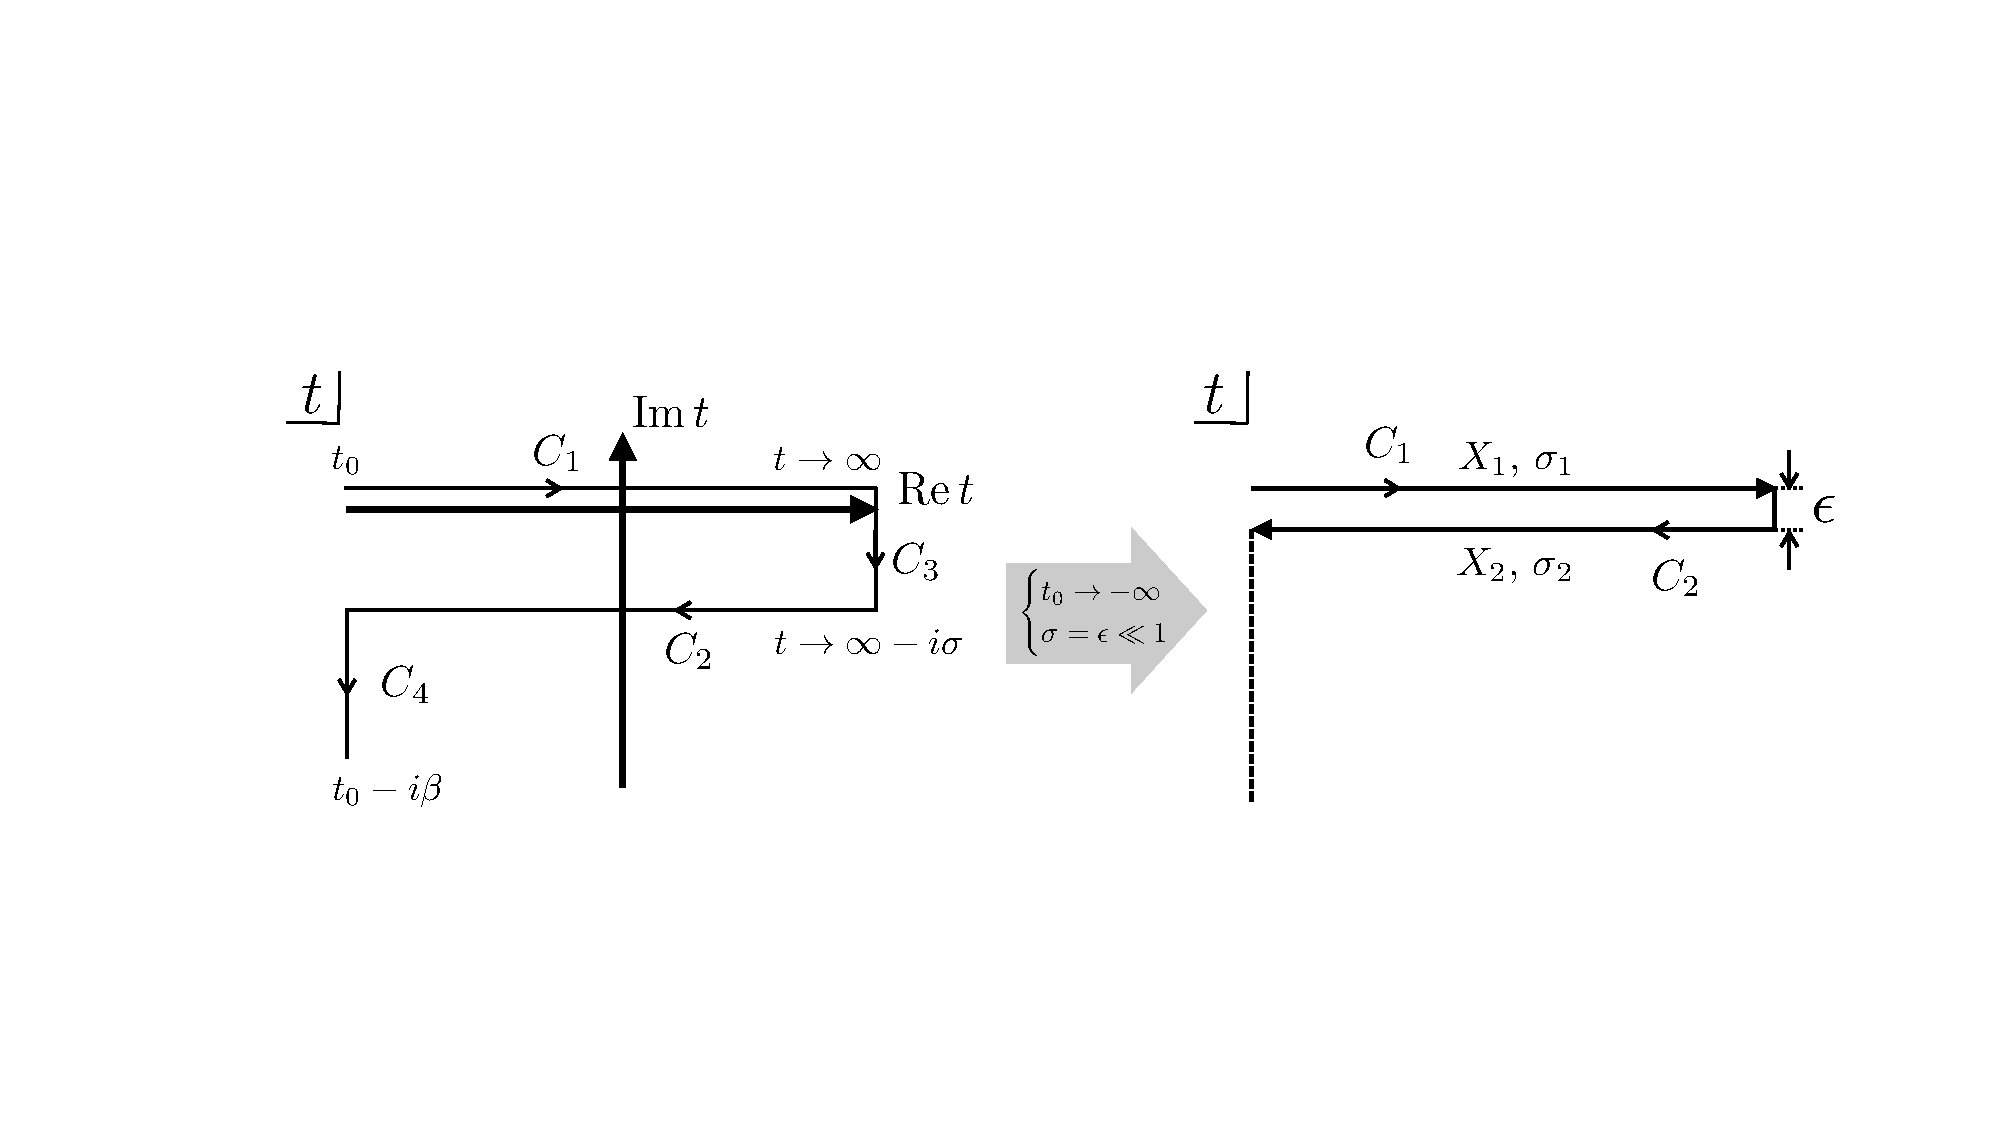
\includegraphics[width=15cm]{original/fig_ctp_ap}
\caption{初期時刻に熱化した系の一般的な閉時間経路（CTP）積分路$C$（左図）から出発し、初期時刻を過去無限遠へ移し（$t_0\to-\infty$）、前進経路と後退経路を互いに重ねる（$\sigma=\epsilon\ll1$）極限（右図）を選ぶ。この極限では、前進経路と後退経路上の変数（それぞれ$(X_1,\sigma_1)$および$(X_2,\sigma_2)$で表される）の間のGreen関数のみを考えればよい。}
\label{app:ctp}
\end{center}
\end{figure}

\medskip
系の有効作用$S_{\mathrm{eff}}[X_1,X_2]$を得るため、まず初期時刻を過去無限遠$t_0\to-\infty$へ移し、パラメータを$\sigma=\epsilon\ll1$と選ぶ（図\ref{app:ctp}右を参照）。これにより、前進積分路と後退積分路$C_{12}\equiv C_1\cup C_2$上の変数間の相関だけを考えればよくなり、問題は大幅に簡単になる。作用は環境$x$について1次および2次の項しか含まないため、有効作用$S_{\mathrm{eff}}[X_1,X_2]$は容易に計算でき、次のようになる。
\begin{align}
\nonumber
& iS_{\mathrm{eff}}[X_1,X_2]
= i \int_{-\infty}^\infty dt \big(L_{\mathrm{sys}} (X_1) -L_{\mathrm{sys}} (X_2)\big)
\\
& \quad\quad - \frac{g^2}{2} \int_{-\infty}^\infty dt \int_{-\infty}^\infty dt'
  \left(\begin{array}{cc}X_1(t) & -X_2(t)\end{array}\right)\left(\begin{array}{cc}G_{11} (t-t') & G_{12} (t-t') \\G_{21} (t-t') & G_{22} (t-t')\end{array}\right)\left(\begin{array}{c}X_1(t') \\-X_2(t')\end{array}\right).
  \label{eq:Seff}
\end{align}
ここで、次のGreen関数の組を導入した。
\begin{align}
\begin{split}
 G_{11}(t- t') &= \theta(t-t') G^> (t-t') + \theta(t'-t) G^< (t-t'),
 \\
 G_{12}(t- t') &= G^{<}(t-t'),
 \\
 G_{21}(t- t') &= G^{>}(t-t'),
 \\
 G_{22}(t- t') &= \theta(t'-t) G^>(t-t') + \theta(t-t') G^<(t-t').
\end{split}
\end{align}
次に、$\rho(\omega)=2\pi\,\mathrm{sgn}(\omega)\delta(\omega^2-\omega_0^2)$を用いると、Fourier空間におけるすべてのGreen関数の具体形を得る。
\begin{align}
\begin{split}
 G_{11} (\omega;\omega_0^2)
 &=  \frac{i}{\omega^2-\omega_0^2 + i \epsilon}
 + 2 \pi n_B (|\omega|) \delta (\omega^2-\omega_0^2)\\
 &=\mathbf{P}\left(\frac{i}{\omega^{2}-\omega_{0}^{2}}\right)
+2\pi{\rm sgn}(\omega)\delta(\omega^{2}-\omega_{0}^{2})\left(\frac{1}{2}+n_B(\omega)\right)  ,
 \\
 G_{12} (\omega;\omega_0^2)
 &= 2 \pi\,\mathrm{sgn} (\omega) \delta (\omega^2-\omega_0^2) n_B (\omega) ,
 \\
 G_{21} (\omega;\omega_0^2)
 &= 2 \pi\,\mathrm{sgn} (\omega) \delta (\omega^2-\omega_0^2)
 \big( 1 + n_B (\omega) \big),
 \\
 G_{22} (\omega;\omega_0^2) &= \big( G_{11} (\omega;\omega_0) \big)^* ,
 \end{split}
 \label{def:Greenfunc}
\end{align}
ここで$\mathbf{P}$は主値を表し、後のために$\omega_0$への依存性を明示した。これらの式により、系の有効作用~\eqref{eq:Seff}における$X_1$と$X_2$の混合項が得られる。これらの項は、環境を積分消去する操作、すなわち粗視化操作の直接的な結果として現れることに注意したい。

\medskip
最後に、単一の調和振動子に対する結果~\eqref{def:Greenfunc}を、複数の調和振動子の場合へ一般化する。これは、次の置き換えによって容易に行える。
\begin{align}
 g^2G_{ab} (\omega;\omega_0^2)
  \to \mathcal{G}_{ab} (\omega)
  \equiv \sum_{n=1}^N g_n^2G_{ab} (\omega;\omega_n^2)\,,
\end{align}
これは、各スケール$\omega$において、環境がBrown粒子の力学に及ぼす効果を特徴づける。特に、大きな$N$の極限、言い換えれば連続スペクトルに関心がある場合には、次式を満たす重み関数$J(\omega_0^2)$を導入すると便利である。
\begin{align}
 \mathcal{G}_{ab} (\omega)
  \equiv \frac{1}{2\pi} \int_{0}^{\Lambda^{2}} d\omega_0^{2}
 J(\omega_0^2) G_{ab} (\omega;\omega_0^2),
 \label{eq:GreenMulticase}
\end{align}
ここで環境の分布に対するカットオフスケール$\Lambda$を導入した。高い振動数$\omega_0\gg T$を持つ調和振動子は熱的にはあまり励起されないため、Brown粒子の力学に及ぼす効果は無視できるであろう。そこで$\Lambda\sim T$と仮定する。

\medskip
以下では、温度スケールに比べて小さい振動数領域$\omega\ll T$に着目し、重み関数が次の形を取ると仮定する。
\begin{equation}
\label{Ohmic}
 \mathrm{sgn}\, (\omega) J(\omega^2)
  = 2\gamma\omega\Big[ 1 + O \left(\frac{\omega^2}{\Lambda^2}\right) \Big],
\end{equation}
ここで$\mathrm{sgn}\,(\omega)J(\omega^2)$は$\omega$の奇関数であるため、$\omega=0$で有限である限り、最低次は1次の項となることに注意したい。この1次の項の係数を$2\gamma$（$>0$）と置く。この係数は質量次元1を持つ（係数2は後の便宜のために付けた）。この重み関数で記述される環境は\textit{Ohmic浴}として知られている~\cite{kamenev2011field}。この場合、式\eqref{eq:GreenMulticase}の$\omega_0^2$積分を実行でき、次を得る。
\begin{equation}
 \begin{split}
\mathcal{G}_{11} (\omega)
  &\simeq \gamma(-iC
  + 2T)\,,
\\
  \mathcal{G}_{12} (\omega)
  &\simeq \gamma(-\omega
  + 2T)\,,
\\
  \mathcal{G}_{21} (\omega)
  &\simeq  \gamma(\omega
  + 2T)\,,
\\
  \mathcal{G}_{22} (\omega) &\simeq\gamma(iC
  + 2T)\,,
\end{split}
\end{equation}
ここで$C=2\Lambda/\pi$を導入し、$\omega/T$展開の高次項を落とした。実時間座標では、次のようになる。
\begin{equation}
 \begin{split}
\mathcal{G}_{11} (t,t') &\simeq \gamma\delta(t-t')\left(- iC
  + 2T\right),
\\
\mathcal{G}_{12} (t,t')& \simeq \gamma\delta(t-t')\left(- i \partial_{t'}
  + 2T\right),
 \\
 \mathcal{G}_{21} (t,t')
 &\simeq \gamma\delta(t-t')\left( i\partial_{t'}
  + 2T\right),
 \\
 \mathcal{G}_{22} (t,t')
 &\simeq \gamma\delta(t-t')\left( iC
  + 2T\right).
\end{split}
\end{equation}
最終的に、有効作用~\eqref{eq:Seff}は次のようになる。
\begin{align}
\nonumber
 iS_{\mathrm{eff}}[X_1,X_2]
&
 =   i \int_{-\infty}^\infty dt \big(L_{\mathrm{sys}} (X_1) -L_{\mathrm{sys}} (X_2)\big)
 \\
&\quad  -\frac{1}{2}
  \int_{-\infty}^\infty dt
 \left[ i\gamma\left(X_1\dot{X}_2-\dot{X}_1X_2\right) +2\gamma T\left(X_1^2+X_2^2-2X_1X_2\right)\right],
\end{align}
ここで定数$C$は、繰り込みによりBrown粒子のポテンシャル$V(X)$に吸収した。$X\to M^{1/2}X$と再スケールすると、有効作用~\eqref{eq:MSR3}が得られる。



\clearpage
\renewcommand{\refname}{\hyperlink{toc}{参考文献}}
\bibliographystyle{utphys}
\bibliography{ref}
\end{document}
